
\documentclass[12pt,a4paper,notitlepage,twoside,openright]{report}
%\documentclass[12pt,a4paper,draft,notitlepage,twoside,openright]{report}

%Libraries for greek
\usepackage{xltxtra}
%\usepackage{xgreek} 
\setmainfont[Mapping=tex-text]{Times New Roman}
%\usepackage{cmap}
%\usepackage{ucs}
%\usepackage{kerkis}
%\usepackage[english,greek]{babel}
\usepackage[utf8x]{inputenc}

\usepackage[colorlinks=true]{hyperref} 					%hyperlinks
\hypersetup{linkcolor=blue,citecolor=blue,linktoc=page} %hyperlink options
\usepackage[a4paper,top=3cm,bottom=2cm,left=3cm,right=3cm,marginparwidth=1.75cm]{geometry}
\usepackage{setspace}
\onehalfspacing
\raggedbottom % disables vertical alignment & stretching
\setlength\parindent{0pt} %me auto den exw esoxes se kamia paragrafo (diladi noindent pantou)
\usepackage[parfill]{parskip}
\usepackage{titlesec}
\titleformat{\chapter}[display]{\normalfont\Huge\bfseries}{\chaptertitlename\ \thechapter}{15pt}{\Huge}
\titlespacing{\chapter}{0pt}{40pt}{21pt}
\titlespacing{\section}{0pt}{0pt}{0pt}
\titlespacing{\subsection}{0pt}{0pt}{0pt}
\titlespacing{\subsubsection}{0pt}{0pt}{0pt}
\usepackage{tocloft}
%\recommand\cftchapafterpnum{\vskip5pt}

\usepackage{fancyhdr} %control of page headers and footers- me auto vazw tis eutheies grammes panw kai katw stis selides
\renewcommand{\footrulewidth}{0.4pt}
%\lhead[\rm \bf \thepage]{\fancyplain{}{\sl{\rightmark}}}
\rhead{\rm \bf \thepage}{\fancyplain{}{\sl{\leftmark }}}
\chead{}\lfoot{}\rfoot{}\cfoot{}

\usepackage{graphicx}
\usepackage{amsmath} %extra math
\usepackage{mathtools}
\usepackage{amssymb} %extra symbols
\usepackage{gensymb}
\usepackage{breqn}  %break equations
\usepackage[notlof,notlot,nottoc]{tocbibind} %bibliography is not a numbered chapter
\usepackage{fixltx2e} %gia na grafw textsuperscript + textsubscript
\usepackage{enumitem} %gia to itemize
\usepackage{relsize} %gia \mathlarger + \mathsmaller
\usepackage{subcaption}
\usepackage{mwe}
\usepackage{siunitx} %gia na xrisimopoiisw to \ang{360}--> gia na valei to symvolo twn moirwn (degree)
\usepackage{textcomp}

\usepackage{algorithm}
\usepackage[noend]{algpseudocode} %gia pseudokwdika- otan thelw na perigrapsw kai kala code

\makeatletter
\def\BState{\State\hskip-\ALG@thistlm}
\makeatother

\usepackage{amssymb}
\usepackage{longtable}

\usepackage{xr}
\usepackage{adjustbox} %auto prepei na kathorizei kai an einai i current page odd or even
\usepackage[margin=4pt,font=normalsize,labelfont=bf,textfont=it]{caption}
%\usepackage{subcaption}
%\usepackage{sidecap}
\usepackage{float}
\usepackage{ragged2e} %gia na kanei fully justified text

\newcommand{\HRule}{\rule{\linewidth}{0.5mm}} % New command to make the lines in the title page

\usepackage{color} 								%hilight pachage
\usepackage[dvipsnames]{xcolor}
\newcommand{\hilight}[1]{\colorbox{yellow}{#1}} %hilight color

\usepackage[hang,flushmargin]{footmisc} %a range of footnote options - noindent
\usepackage[normalem]{ulem} %Gia na kanw underline kapoio text
\usepackage{esvect} %For vector with dot

\renewcommand{\figurename}{Fig.} %Ti leei otan vazw eikones (Fig.1 ...)
\renewcommand{\contentsname}{Table of Contents}
\renewcommand{\chaptername}{Chapter}
\renewcommand{\tablename}{Tab.} %Ti leei otan vazw tables (Capt.1 ...)

%% FOR MATLAB CODE
\usepackage{listings}
\usepackage{color} %red, green, blue, yellow, cyan, magenta, black, white
\definecolor{mygreen}{RGB}{28,172,0} % color values Red, Green, Blue
\definecolor{mylilas}{RGB}{170,55,241}

\renewcommand\bibname{References} %If I don't use it, then instead of the name "References", it will say "Bibliography"

%Package for list of acronym in the end of the document
\usepackage{enumitem}
\newlist{abbrv}{itemize}{1}
\setlist[abbrv,1]{label=,labelwidth=1in,align=parleft,itemsep=0.1\baselineskip,leftmargin=!}

\usepackage{flafter} % Not to let the images and the stuff be presented in the document before their actual reference

\begin{document}
\pagenumbering{roman} \pagestyle{plain}
\thispagestyle{empty}
\begin{minipage}{0.2\textwidth}

\includegraphics[width=\textwidth]{./Images/ESA-logo-and-wordmark.png}
\end{minipage}
\begin{minipage}[r]{0.5\textwidth}
\begin{center}
\hspace*{0.5cm}  \Large {\color{Violet}    }\large \\
\hspace*{0.5cm}  {\color{Violet}       } \\
\end{center}
\end{minipage}
\begin{minipage}[r]{0.2\textwidth}

\includegraphics[width=\textwidth]{./Images/TU-Muenchen.png}
\end{minipage}
\begin{minipage}[r]{0.1\textwidth}

\includegraphics[scale=0.13]{./Images/Department_logo.png}
\end{minipage}

\bigskip
\begin{minipage}{0.62\textwidth}
\begin{flushleft}
\normalsize{European Space Agency \\European Space Operations Centre (ESOC) \\Space Debris Office}
\end{flushleft}
\end{minipage}
\begin{minipage}{0.37\textwidth}
\begin{flushleft}
\normalsize{Technische Universität München \\Fakultät für Luftfahrt, Raumfahrt und Geodäsie \\Lehrstuhl für Astronomische und Physikalische Geodäsie }
%\\Univ.-Prof. Dr.techn. Mag.rer.nat. Roland Pail
\end{flushleft}
\end{minipage}

\vspace{3cm}
\begin{center}
\Large{\textbf{Addressing space infrastructure needs and utility on the example of Earth observation satellites \\- \\}}
\Large{\textbf{Potential ways to reduce space traffic by sharing resources}}
% or --> Potential ways to reduce space traffic - Addressing space infrastructure needs and utility on the example of Earth observation satellites
% or --> Addressing space infrastructure needs and utility - potential ways to reduce space traffic on the example of Earth observation satellites
\end{center}
\vspace{2.1cm}
\begin{center}
\large{Master Thesis of:\\
\textit{\textbf{Styliani Konstantinidou}} \\}
\vspace{1cm}
\large{Master's Course in Earth Oriented Space Science and Technology}
\end{center}

\vspace{2.5cm}
\begin{flushleft}
\large{Supervisors: Dr. Vitali Braun \\ \hspace*{2.7cm}Prof. Urs Hugentobler}
\end{flushleft}

\vfill
\begin{center}
\normalsize Munich, 2020
\end{center}



%Abstract
\newpage \mbox{} %mbox-> creates a box just wide enoigh to hold the text in his arguments
\newpage \mbox{}
\thispagestyle{empty}
%\vspace{\fill}
\begin{center}
\Large{\textbf{Abstract}} 
\end{center}
\bigskip
\par 	
The motives of this thesis were the growing numbers of objects in space and the potential to exceed the carrying capacity in the near-Earth orbits. These are addressed by running a first experiment with the software written during this thesis, which can give the incentives to create space traffic management rules based on the orbit and capacity allocation, as well as the added value that each new satellite may have. An attempt to approach its development is to focus on Earth Observation (EO) satellites at LEO. Some capabilities of the software are the calculation of the revisit time of a single satellite or of a constellation at the equator or at a latitude of interest to the user, and the investigation of the orbital characteristics of a satellite in order to achieve a more frequent revisit time together with a group of satellites. Overall, those satellites, which can achieve a significant increase of the revisit rate, have a higher added value compared to other satellites/ mission, which do not come with any considerable changes. The creation of a database of EO satellites connected to the software increased the capabilities of the software, since a user can also find out whether there are operational satellites offering a specific service. For the development of the software, the necessary input data are the TLE set of the satellite, as well as the parameters related to the satellite’s EO sensor, such as the swath width, operational lifetime, spatial resolution and other. Having these parameters, the position of the sub-satellite’s points on Earth is found and based on the swath width the revisit time of the satellite is calculated. The experiments and results showed that higher revisit rates can be achieved when adding a satellite in the same orbital altitude and not placing it in a higher or lower one. Moreover, the addition of a single satellite to an already large constellation does not result in a significant reduction of the revisit time.

Keywords: revisit time, database, classification, added-value, Earth Observation satellites, LEO

%Abstract should give the “Big Picture” of your work
%Should inform the reader (say in 300 words) about: the goal of the work, applied methodology, result of the work
% 

%---------------------------------------------------------------------------
%Acknowledgments
%\newpage \mbox{}
\newpage \mbox{}
\thispagestyle{empty}
%\vspace{\fill}
\Large{\textbf{Acknowledgments}} 
\par
\bigskip
\normalsize I would like to thank Dr. Vitali Braun for having included me in this exciting topic and for his thoughtful supervision. Despite this unprecedented and unstable period, his support was valuable, which kept my interest undimmed and his guidance is truly appreciated.

Additionally, I am also thankful to Prof. Urs Hugentobler for his help and his precious advice. The received feedback was always immediate and constructive.

Finally, my thoughts go to my family and friends, for their much appreciated affection and love.


\vspace{\fill} %\vspace{\fill} in a paragraph will add the filling vertical space below the line in which it eventually appears;

%Declarations
\newpage \mbox{}
\renewcommand{\abstractname}{\Large{{ }}}
\begin{abstract}
\vspace{14cm}
{\it
\noindent
This thesis is a presentation of my original research work. Wherever contributions of others are involved, every effort is made to indicate this clearly, with due reference to the literature, and acknowledgement of collaborative research and discussions.}
\vspace{2cm}
\begin{center}
{\it 
Munich, December 22, 2020}
\end{center}
\begin{center}
\vspace{0.5cm}
{\it
Styliani Konstantinidou \vspace{0.3cm}
\begin{figure}[h]
\centering

\includegraphics[width=0.3\textwidth]{Images/23600678_10155917223598909_906035917_o.png}
\end{figure}}
\end{center}
\end{abstract}



\newpage \mbox{}
\tableofcontents

\newpage \mbox{}
\listoffigures
%\addcontentsline{toc}{chapter}{List of figures} %In order to add it on the "Table of Contents"

\newpage \mbox{}
\listoftables

\clearpage \pagenumbering{arabic} \pagestyle{fancy} %to fancy pagestyle einai auto pou vazei tis eutheies grammes panw kai katw apo tis selides!
\chapter{Introduction}
\lhead{Chapter 1 \emph{Introduction}}
\label{chap:1}
%\autoref{chap:1}

\section{Motivation}
\bigskip
\bigskip

In 1957 the first satellite in history was launched and since then thousands other objects were placed into orbit. \cite{Belward 2015}, \cite{ESA 2019} Two decades later NASA’s scientist Kessler proposed a scenario, in which he theorized that the increasing density of the objects in the Low Earth Orbit (LEO) cause collisions and the generated space debris increase even more the probability of further collisions. The humanity today is confronted more than ever with the realization of this theory, which has gone down as Kessler Syndrome.

There have been taken many important steps towards raising the consciousness about the overpopulation problem, as well as the enactment of rules regarding the capacity and orbit allocation. However, despite the fact that coordination committees and working groups have been established and they are involved in the mitigation guidelines, the existed space traffic management rules deals today only with the frequency allocation used by satellites.

Having said that, the motivation of this thesis is the creation of an application, which will help into supplementing the space traffic management rules regarding the physical location of satellites based on the added value that each satellite contributes to the society in terms of additional services or data. This application is focused on Earth Observation (EO) satellites at LEO, which is one attempt to approach and tackle the problem. In conjunction with a database, which hosts information about the EO satellites that are currently on orbit at LEO, the application also offers the following service. The user can find out about the existing orbiting and operational EO satellites or constellations that provide the outcome/ service that he/she asked for.

\bigskip
\bigskip

\newpage
\section{Scope and key assumptions}
\bigskip

%\textit{Edit it...}

The first part of this work pertains to the Theoretical Framework of the discussed problem; the overpopulation. The points being addressed are: the problem of overpopulation, the concept of orbital capacity, the state of LEO and its critical regions, the basic characteristics of LEO, the different ways of dealing with the problem, as well as the mitigation guidelines, which have been already put into action.

The second part of this master thesis is dedicated to the development of an application, which can give the incentives to create space traffic management rules based on the orbit and capacity allocation, as well as the added value that each new satellite provides. More specifically, the concept of added value is based on the idea that each new satellite is prioritized to be launched when it provides some additional services or data to the society, which are not offered from another existing and functional satellite/ constellation.
%It is not monetary.

An attempt to approach the development of such application is to focus on Earth Observation (EO) satellites at LEO. The reason behind the selection of EO as the first group of satellites to be tested in the application, is because the calculation of the capabilities of an EO satellite is more apparent in comparison to other scientific or technological missions. The same applies to telecommunication missions, due to the fact that there is a competition between the satellite and terrestrial industry and thus it is more complex to estimate the added value that each satellite provides to the society. All things considered, this application focus on EO satellites in LEO and has three main capabilities.
%One should also calculate the bandwidths, apart from the coverage, in the case of the Communication Satellites.

\begin{itemize}
\item The first capability is that the user can define a satellite mission or constellation, which means that the number of satellites, the altitude, the orbital plane, resolution etc. is known. Then, the software can answer what is the revisit time of that defined mission in a certain area.
\item The second capability is the following: The actual outcome/service of a Earth Observation satellite is defined. Namely, if such is images from the visual band of entire Earth, which have a certain revisit time and resolution, then the software can provide to the user the orbital characteristics of the satellite or constellation that can supply the desired data.
\end{itemize}

An extension of this application and its capabilities is the creation of a small database of Earth Observation satellites.

\begin{itemize}
\item In both mentioned capabilities of the application, the user can find out, if there are currently satellites which offer the desired data that they had asked for and if such satellites exist, to name them.
\end{itemize}

The database contributes greatly to the creation of a well-rounded application, which can help into mitigating the problem of overpopulation. Since the user can find out about whether existing satellites do a certain/asked project or offer a specific service, thus he/she can decide whether a new satellite is needed to be launched based on whether the desired service is offered or not by someone else. In this way, it can also incentivize and encourage in the future companies to cooperate with each other, instead of constructing/ designing/ launching a new constellation. Thus, a rule in the field of space traffic management can be formulated based on the added value that a new satellite offers.
%For example, if you define a satellite and this exists in the database, then the value for competition is high, but there is no value for the environment.

The concept of prioritization of the missions based on the additional services that they offer before being launched seems very promising. So, one objective of this thesis is to create awareness among the space industry and the society. Another one is the contribution to the generation of a common ground, which will lead to the formation of legislation based on the added value of the satellites. Hence, consensus in the corresponding committees can be reached and the mitigation of the problem of overpopulation by attenuating the number of satellites that are launched can be actualized.


%A space traffic management application towards the estimation of added value.

%Lastly, the part of the Evaluation follows, as well as parts of Summary and Conclusions and that of Future work.



\bigskip
\section{Current launching trend}
\bigskip

%Current launching trend

Having said that, the current trend is that the world goes in the direction of launching more and more small satellites, which are most of the times parts of large constellations aiming at providing persistent global internet. The reason that lies behind is that the commercial space industry has benefits such low costs and increased competition. Nevertheless, the notion of proliferated constellations is propitiatory for the future. This is because it provides more resilience, since the loss of a satellite will not hamstring the whole constellation and the mission can continue.

(especially in LEO)
(Fig. \ref{launch_traffic_LEO}) (Fig. \ref{launch_traffic_GEO}) 

\begin{figure}
\centering
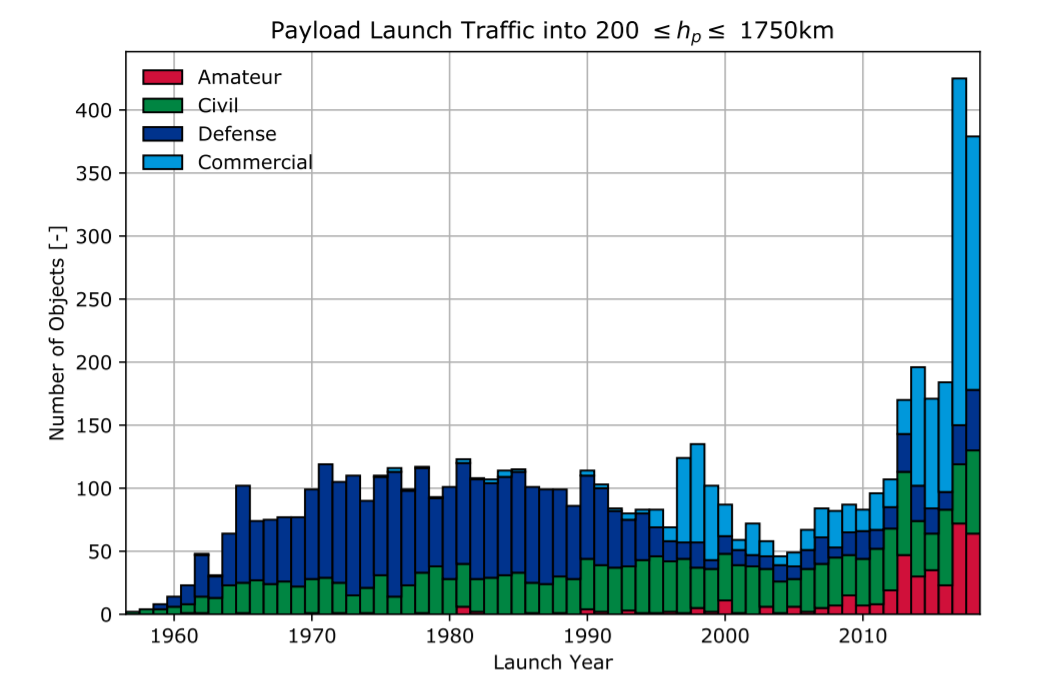
\includegraphics[width=0.9\textwidth]{Images/launch_traffic_LEO.png}\caption{Payload launch traffic into LEO (1957-2019). \textit{Source: \cite{ESA 2019}}}
\label{launch_traffic} 
\end{figure}

\begin{figure}
\centering
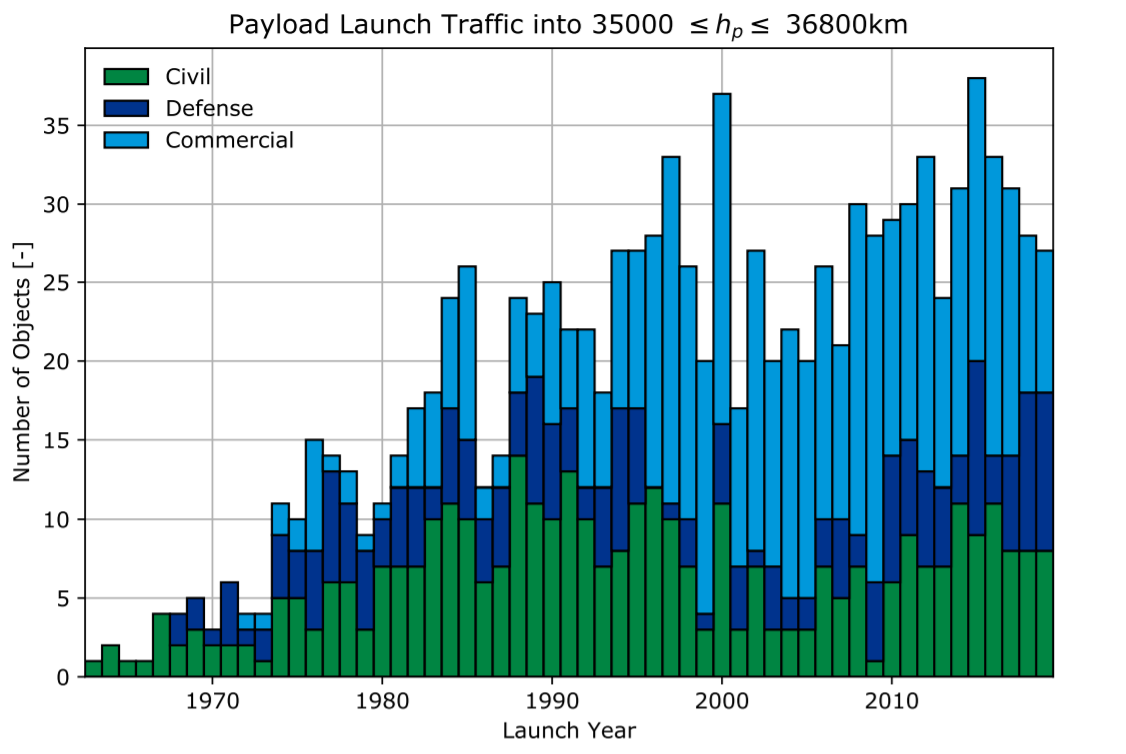
\includegraphics[width=0.9\textwidth]{Images/launch_traffic_GEO.png}\caption{Payload launch traffic into GEO (1957-2019). \textit{Source: \cite{ESA 2019}}}
\label{launch_traffic} 
\end{figure}

It seems that space nowadays can be linked to the phenomenon of Tragedy of Commons. Based on this concept written by the British economist Lloyd, the shared-resource system is spoiled by individual users who act based on their own benefit and against the common good. This notion describes the current situation of the space industry. +++ non-infinite environment +++ At the same time the "no ownership in space" gave the permission to people....

%the current situation of the big constellations (e.g. Starlink) --> mention that is happening, but now the focus is on EO (for the above reasons)

%Soon space will reach the capacity limits - too many satellites. This will fuel the space debris. (here or Chapter 2?)
%Space sustainability! -check space sustainability rating- I have googled it.

% (this goes to Intro... Some say that we can avoid all collisions. But, can we? There are sensitivy limits in the instruments, such as radars, telescopes. You can't detect objects in the mm scale. But, if you control it and have less debris, then you have less risk.

%New Space community - what is it? (more satellites transmittance or ...?"

%One question: "I want a certain EO task" --> What resolution can I have without exceeding orbit capacity?"
\chapter{Theoretical Framework}
\lhead{Chapter 2 \emph{Theoretical Framework}}
\label{chap:2}
%\autoref{chap:2}

\section{The problem of overpopulation}
\bigskip

%(Kind of intro about ways to deal?) The first accidental collision took place in 2009 between two communications satellites, the US commercial non-operational Iridium 33 and the Russian military Kosmos-2251. The number of debris that this collision left behind was 1,366 pieces with average size of 12.5cm and average weight 1.1kg. \cite{Kelso 2009}
It is benchmark 

%The problem of overpopulation and of the increasing number of space debris is that the possibility of impact between a debris and an operational functioning orbiting object is very high. --> Edw mention Letizia space 

%Vale orbital capacity (Vale san section? Giati to exw an aferei sto 1.2 Scope etc.)
+ Look for certain - long term environmental similarities. They look how the same number change (?) if the growth continues (?). How many missions are added in the space debris? Compute capacity for certain mission. Low reliability  == More capacity.

%Rules? e.g. Every orbital plane has a certain capacity. Based on those, the future satellite constellations should work. In general, there are no rules about the capacity allocation!

---------------

\section{LEO: a favorable spot}
\bigskip
%LEO Low Earth Orbit. (Overview - Status?!)

The Low Earth Orbit (LEO) is a favorable spot for placing satellites for various reasons. It's proximity from Earth makes it possible to launch even CubeSats, since their fuel capacity is enough to be able to maintain their position and/or to de-orbit at the end of their mission. Specifically in the recent years more and more small satellites and/or CubeSats are placed in LEO and in large constellations. (Fig. \ref{launch_traffic_LEO}) The need of proliferated constellations is also linked to the low altitude of the LEO region. Namely, for larger coverage, a satellite should be either placed in a higher altitude, or the mission should engage more satellites in order to compensate the smaller field of view that one satellite offers.

++ The total number of operating satellites, as of 31.3.2020 including all the launches by that date is 2,666 with 1,918 being in LEO. \cite{UCS} 

**• Launch traffic into the LEO protected region is changing significantly, fuelled by the proliferation of small
payloads, i.e. below 10.0 kg in mass, during the last few years in terms of number, but not contributing
significantly to the mass. (ESA report p.77)

\begin{figure}
\centering
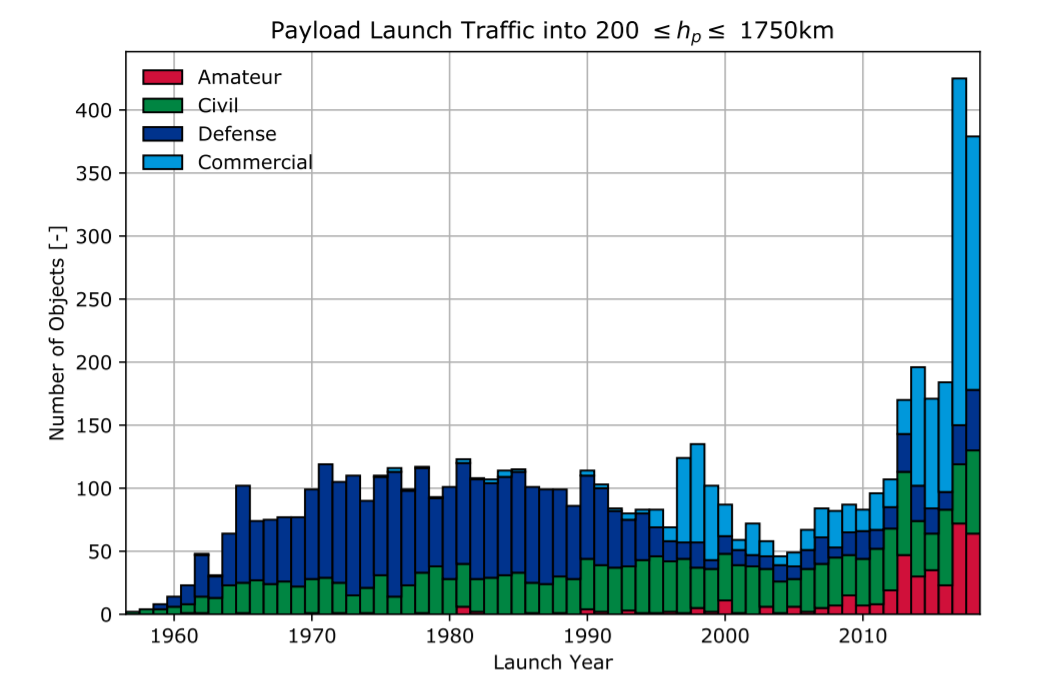
\includegraphics[width=0.9\textwidth]{Images/launch_traffic_LEO.png}\caption{Payload launch traffic into LEO (1957-2019). \textit{Source: \cite{ESA 2019}}}
\label{launch_traffic} 
\end{figure}

((Having said that, the current trend is that the world goes in the direction of launching more and more small satellites.))
This situation happens regardless of the overpopulation issues that exist in some regions of LEO, which has already been declared as critical. More specifically, the three critical regions in LEO are \cite{Kramer 2002}:
\begin{itemize}
\item The first critical region is at the altitude 750-850km, at which the spatial density is increased because of the debris' population. It is characterized as critical, because objects need hundreds of years in order to decay and re-enter the atmosphere.
\item The second critical region is at the altitude 900-1000km, at which there is a high number of massive objects. Drag is also not sufficient in order to help objects decay and thus the spatial density increases over time.
\item The third critical region is at the altitude 1100-1300km. At this region the effect of drag is negligible, which means that any additional object builds up the orbital population.
%The future large constellations will be placed around these altitudes, which makes this region even more alarming. \cite{Somma 2019}
\end{itemize}

%%Some general things about LEO:
%	General altitude range: 160-2000km above Earth’s surface.
%	Orbital periods between 88-127 min.
%	All inclinations possible
%	Orbital velocity (with regard to an observer on Earth): 7-8km/s
%	LEO subclasses/ “shapes”:
%•	Circular LEO orbit is the most common and natural orbit for Earth observation, especially in the altitude range of about 200-900 km with orbital periods of about 90-105min.
%•	Special orbits:
%	Polar orbit
%	Sun-Synchronous orbit (a special case of near-polar orbit!):
%An orbit like this is possible by the fact that the Earth is not a perfect sphere. In the SSO, the daily rotation of the orbital satellite plane (with respect to the equatorial plane) is identical to the mean motion of the fictitious sun around the Earth = which is identical to the mean motion of the Earth around the sun.
%	Check the relationship between the coverage and revisit/ repeat period with the inclination and altitude. (It’s on the application’s part.)


\subsection{Critical regions of LEO}
\bigskip

\section{Mitigation principles}
\bigskip

There have been made many important steps towards raising the consciousness about the overpopulation problem, as well as the enactment of rules regarding the capacity and orbit allocation. In 1993 the Inter-Agency Space Debris Coordination Committee (IADC) was founded. Some years later, in 2002 IADC published for the first time a report about Space Debris Mitigation Guidelines. These guidelines were presented at the United Nations Committee on the Peaceful Uses of Outer Space (UNCOPUOUS), which is a committee established by United Nations Office for Outer Space Affairs (UNOOSA). In 2003 another group working towards similar goals was created – the Orbital Debris Co-ordination Working Group (ODCWG), which was created by unanimous agreement of International Organization for Standardization (ISO). \cite{Klinkrad 2006}

Even though there are working groups (UNCOPUOUS, ODCWG) dealing with the mitigation guidelines, currently the existed space traffic management rules deal only with the frequency allocation used by satellites. For this reason, the motivation of this thesis is the creation of an application, which will help into supplementing the space traffic management rules regarding the physical location of satellites and the value added that they will contribute once launched.



--International cooperation at a technical level --
IADC (Inter-Agency Space Debris Coordination Committee) has declared protected regions \cite{IADC 2007}. "an inter-governmental forum whose aim is to co-ordinate efforts to deal with debris in orbit around the Earth founded in 1993." (It is composed of space agencies..)
%cite Space Debris: Models and Risk Analysis (978-3-540-37674-3) 


-- International standards and policies --
IADC also occupies a crucial role as a technical specialized group in the field of space debris since it supports the UNCOPUOUS.
The first publication related to the space debris mitigation was performed in 2002 by IADC and presented at UNCOPUOUS in 2003.

[[---> Also IADC guidelines (The UN Space Debris Mitigation Guidelines) --> Drafted on request of UNCOPUOUS (United Nations Committee on the Peaceful Uses of Outer Space), which is a committee established by UNOOSA (United Nations Office for Outer Space Affairs). \cite{IADC 2007}
1. Prevent the release of mission related object
2. Implement collision avoidance measures
3. Disposal
4. Passivation
5. Limit on-ground risk due to re-entry]]

The two main groups that they work towards these goals are the UNCOPUOUS working group and the Orbital Debris Co-ordination Working Group (ODCWG), which was created in 2003 by unanimous agreement of the ISO (International Organization for Standardization).

[[The recognized concepts from this meeting was that the mitigation of Orbital Space Debris is of international concern and the ISO is responsible for developing standards on a consensus basis.]]


\chapter{Methodology}
\lhead{Chapter 3 \emph{Methodology}}
\label{chap:3}
%\autoref{chap:3}

% How I did it? First part of application by having the keplerian elements ....
% The implementation was done using Python and PostgreSQL (?)
%Print earth map. Based on the FOV and the revisit frequency, I can see how the Earth will be printed/colored (heat map). So, we want to track coverage/ revisit time across the equator.

% Tip: "Do not present data at this stage but use sketches or synthetic data instead"

% The app is used for analysis. It is not opeartional (obviously), so no need to check for mistakes in the import of the parameters.

% In the part of the database: mention that we focus on LEO and EO satellites!


\section{Sources of data}
\bigskip

\section{Data gathering procedure}
\bigskip

\section{Data analysis}
\bigskip

%Add a chapter "Results"???
\chapter{Evaluation \& Discussion}
\lhead{Chapter 4 \emph{Evaluation}}
\label{chap:4}
%\autoref{cha:4}

\section{}
\bigskip

% Another chapter is: EXPERIMENTS AND RESULTS??

% -- Present your data and test area
% -- Indicate the parameters and setting you have used
% -- Show the results without judging them
% -- Present your evaluation method and its outcomeexample: accuracy assessment

% So, maybe another chapter will be for "Evaluation and Discussion" ??


%The discussion will consist of argumentation. In other words, you investigate a phenomenon from several different perspectives. To discuss means to question your findings, and to consider different interpretations. Here are a few examples of formulations that signal argumentation:
%
%On the one hand … and on the other …
%However …
%… it could also be argued that …
%… another possible explanation may be …

% In the evaluation part:
-- Judge your results critically
-- Compare your results with the results form other methods/works/experiments (keyword: validation)
-- show problems

% I will test the software with the big and well-known satellites, like Sentinel-1. 
%\chapter{Summary \& Conclusions}
\lhead{Chapter 5 \emph{Summary \& Conclusions}}
\label{chap:5}
%\autoref{chap:5}

% I should also mention about the further work that can be done or in a seperate chapter "Outlook" !
--  Suggest possibilities for further developments and tests
--  Present other remarks for future work: prioritization of the missions based on the added value in the society. So say that this work has helped into this direction...

-- Outlook:
The application can be further expanded in order to offer more capabilities. Practically: The heat map that was presented in the first part of the application, will also have a 3rd dimension, in which it will show the time that the satellite has passed from every spot of the Earth. The benefit of that will be that when the user will specify a certain area of interest then, the orbits of various satellites can be calculated and then based on the time that each satellite passes, it can be found whether there are some common periods that the satellites pass from the same area at the same (or almost the same) time. 
(So far -in the first part of the application- there is only a count when a satellite passes from an area. In this aforementioned idea, the exact time will be saved.)
This idea came from the Cryo2Ice mission * Find source :https://www.bbc.com/news/science-environment-53326490

\newpage
%\chapter*{References}
%\lhead{\emph{References}}
%\label{ref}



\chapter*{List of acronyms}
\addcontentsline{toc}{chapter}{List of acronyms}
\begin{abbrv}
% American Institute of Aeronautics and Astronautics (AIAA)
\item[\textit{ASI}] Agenzia Spaziale Italiana - Italian Space Agency
\item[\textit{CONAE}] Comisión Nacional de Actividades Espaciales of Argentina - \newline Argentinian Space Agency
\item[\textit{DMF}] Debris Mitigation Framework
\item[\textit{ECSS}] European Cooperation for Space Standardization
\item[\textit{EO}] Earth Observation
\item[\textit{EU}] European Union
\item[\textit{GEO}] Geostationary Orbit / Geosynchronous Equatorial Orbit
\item[\textit{GEOSS}] Global Earth Observation System of Systems
\item[\textit{GLAS}] Geoscience Laser Altimeter System
\item[\textit{HRMS}] High Resolution Multi-Spectral
\item[\textit{HSIS}] Hyper Spectral Image Simulator
\item[\textit{IADC}] Inter-Agency Space Debris Coordination Committee
\item[\textit{ISO}] International Organization for Standardization
\item[\textit{ISS}] International Space Station
\item[\textit{LE}] London Economics
\item[\textit{LEO}] Low Earth Orbit
\item[\textit{MELVO}] Moderately Elliptical Very Low Orbit
\item[\textit{MSI}] Multi-Spectral Imager
\item[\textit{MSS}] Multi-Spectral Imaging System
\item[\textit{MSU}] Multi-Spectral Scanner Unit
\item[\textit{MUXCam}] Multi-Spectral Camera
\item[\textit{NIR}] Near Infrared
\item[\textit{ODCWG}] Orbital Debris Co-ordination Working Group
\item[\textit{OECD}] Organization for Economic Co-operation and Development
\item[\textit{PAN}] Panchromatic Imager
\item[\textit{SAR}] Synthetic Aperture Radar
\item[\textit{SIRAL}] SAR Interferometry Radar Altimeter
\item[\textit{SSO}] Sun-Synchronous Orbit
\item[\textit{SSR}] Space Sustainability Rating
\item[\textit{SWIR}] Short-Wave Infrared Light
\item[\textit{UN}] United Nations
\item[\textit{UNCOPUOUS}] United Nations Committee on the Peaceful Uses of Outer Space
\item[\textit{UNOOSA}] United Nations Office for Outer Space Affairs
\item[\textit{VNIR}] Visible and Near-infrared
\item[\textit{WEF}] World Economic Forum
\item[\textit{WFI}] Wide Field Imager
\item[\textit{WPM}] Wide Swath Panchromatic \& Multispectral Camera
\end{abbrv}


\begin{thebibliography}{100}
\bigskip

\bibitem{Cryo2ice_news} Amos J (2020) ESA and NASA line up satellites to measure Antarctic sea-ice. BBC News. Available at: https://www.bbc.com/news/science-environment-53326490 (Accessed July 30, 2020)
\bibitem{Cosmos} Battagliere ML, Daraio MG, Lenti F, Pisani AR, Coletta A (2018) Cosmo-Skymed and the ASO-CONAE cooperation: The SIASGE Programme. 68th International Astronautical Congress (IAC), Bremen, Germany, 1-5 October 2018.
\bibitem{Belward 2015} Belward AS, Skøien JO (2015) Who launched what, when and why; trends in global land-cover observation capacity from civilian earth observation satellites. ISPRS Journal of Photogrammetry and Remote Sensing, May; 103: 115–128.
\bibitem{Blake} Blake JA, Chote P, Pollacco D, Feline W, Privett G, Ash A, Eves S, Greenwood N, Marsh TR, Veras D, Watson C (2020) DebrisWatch I: A survey of faint geosynchronous debris. Advances in Space Research
\bibitem{Amazon} Boyle A (April 4, 2019) Amazon to offer broadband access from orbit with 3,236-satellite ‘Project Kuiper’ constellation. GeekWire. Available at: https://www.geekwire.com/2019/amazon-project-kuiper-broadband-satellite/ (Accessed July 1, 2020)
\bibitem{Braun} Braun V, Lemmens S (2020) Addressing space debris mitigation in satellite mission design. 71st International Astronautical Congress (IAC) – The CyberSpace Edition, 12-14 October 2020
\bibitem{Cadman} Cadman J (May 18, 2020) Op-ed | An unexpected effect: the industry’s recent challenges prove the importance of space. Space News. Available at: https://spacenews.com/op-ed-an-unexpected-effect-the-industrys-recent-challenges-prove-the-importance-of-space/ (Accessed July 1, 2020)
\bibitem{Campbell} Campbell BA, McCandless PW (1996) Introduction to space sciences and spacecraft applications. Elsevier
\bibitem{Committee 2019} Committee on the Peaceful Uses of Outer Space (2019) The “Space2030” Agenda: Space as a driver of sustainable development, Vienna, Report No.: 28th.
\bibitem{Crisp 2020} Crisp NH, Roberts PC, Livadiotti S, Oiko VTA, Edmondson S, Haigh SJ, Huyton C, Sinpetru LA, Smith KL, Worrall SD, Becedas J (2020) The benefits of very low earth orbit for earth observation missions. Progress in Aerospace Sciences, 117, p.100619.
\bibitem{Anti-satellite} David L (Feb 2, 2007) China's Anti-Satellite Test: Worrisome Debris Cloud Circles Earth. SPACE.com [Internet] Available at: https://www.space.com/3415-china-anti-satellite-test-worrisome-debris-cloud-circles-earth.html (Accessed July 1, 2020)
\bibitem{Erwin} Erwin S (May 18, 2020) SpaceX rideshare program putting downward pressure on prices [Internet]. Space News. Available at: https://spacenews.com/spacex-rideshare-program-putting-downward-pressure-on-prices/ (Accessed July 1, 2020)
\bibitem{cooperation} ESA (2020) New space satellite pinpoints industrial methane emissions. Available at: https://www.esa.int/Applications/Observing_the_Earth/Copernicus/Sentinel-5P/New_Space_satellite_pinpoints_industrial_methane_emissions (Accessed October 30, 2020)
\bibitem{ESA EO} ESA Space Solutions (August 11, 2020) Newcomers Earth Observation Guide. Report Version 1.9 Available at: https://business.esa.int/newcomers-earth-observation-guide (Accessed November 1, 2020)
\bibitem{ESA 2020} ESA Space Debris Office - ESOC, (Sep 2020) ESA’s Annual Space Environment Report [Internet]. Report No.: 4.0, p. 88. Available at: https://www.sdo.esoc.esa.int/environment_report/Space_Environment_Report_latest.pdf
%Statistics: https://sdup.esoc.esa.int/discosweb/statistics/
\bibitem{LE_Esteve} Esteve R (2020) Earth Observation: a tool for a more resilient and sustainable world? London Economics: Space In Focus, Issue 2
\bibitem{Space sustainability} Foust J (May 7, 2019) Consortium to develop “space sustainability” rating system. Space News. Available at: https://spacenews.com/consortium-to-develop-space-sustainability-rating-system/ (Accessed July 1, 2020)
\bibitem{Griffin} Griffin M (2010) Orbit/Spectrum Allocation Procedures. Space Services Department ITU Radiocommunication Bureau (BR) Conference of ITU in Bangkok, Thailand
\bibitem{Hallex} Hallex MA, Cottom TS (2020) Proliferated Commercial Satellite Constellations - Implications for National Security. Joint Force Quarterly (JFQ) 97
\bibitem{Kepler} Henry C (August 29, 2018) Kepler Communications opens launch bids for Gen-1 LEO constellation. Space News. Available at: https://spacenews.com/kepler-communications-opens-launch-bids-for-gen-1-leo-constellation/ (Accessed July 2, 2020)
\bibitem{Viasat} Henry C (April 24, 2020) Viasat gets FCC approval for MEO constellation. Space News. Available at: https://spacenews.com/viasat-gets-fcc-approval-for-meo-constellation/ (Accessed July 1, 2020)
\bibitem{IADC 2007} Inter-Agency Space Debris Coordinate Committee (IADC) -  Steering Group and Working Group 4 (2007) IADC Space Debris Mitigation Guidelines. Report No.: 22.4. Revision 1
%Available at: https://www.unoosa.org/documents/pdf/spacelaw/sd/IADC-2002-01-IADC-Space_Debris-Guidelines-Revision1.pdf
\bibitem{Kelso 2009} Kelso TS (2009) Analysis and Implications of the Iridium 33-Cosmos 2251 Collision. InAdvanced Maui Optical and Space Surveillance Technologies Conference
\bibitem{Klinkrad 2006} Klinkrad H (2006) Space Debris: Models and Risk Analysis. Springer Verlag, 1st ed., p.430
\bibitem{Klinkrad 2009} Klinkrad H, Johnson NL (2009) Space debris environment remediation concepts. 5th European Conference on Space Debris. In Darmstadt, Germany; (ESA SP-672). 
\bibitem{Kramer 2002} Kramer H (2002) Observation of the Earth and its Environment. Springer Verlag, 4th ed., p.1514, Updated version: Apr, 2020 Available at: https://directory.eoportal.org/web/eoportal/kramer
\bibitem{Newspace} Kulu E (2020) NewSpace Index - Overview of commercial satellite constellations. [Database] Available at: https://www.newspace.im/
\bibitem{Lapaine} Lapaine M, Usery EL (2017) Choosing a map projection. Cham: Springer
\bibitem{Letizia 2019} Letizia F, Lemmens S, Bastida Virgili B, Krag H. (2019) Application of a debris index for global evaluation of mitigation strategies. Acta Astronautica. 161:348–62.
\bibitem{Luo} Luo X, Wang M, Dai G, Chen X (2017) A novel technique to compute the revisit time of satellites and its application in remote sensing satellite optimization design. International Journal of Aerospace Engineering
\bibitem{Oneweb_bankruptcy} Malik T (March 28, 2020) OneWeb, a satellite internet startup, files for Chapter 11 bankruptcy. SPACE.com [Internet] Available at: https://www.space.com/oneweb-satellite-internet-startup-files-for-bankruptcy.html (Accessed July 1, 2020)
\bibitem{Meseguer} Meseguer J, Pérez-Grande I, Sanz-Andrés A (2012) Keplerian orbits - Spacecraft thermal control. Elsevier p.39-57
\bibitem{Satellogic} Mohney D (January 16, 2019) Satellogic signs launch contracts for 90 imaging satellites. Space It Bridge. Available at: https://www.spaceitbridge.com/satellogic-signs-launch-contracts-for-90-imaging-satellites.htm (Accessed July 1, 2020)
\bibitem{Montenbruck} Montenbruck O, Gill E, Lutze F (2002) Satellite orbits: models, methods, and applications. Appl. Mech. Rev., 55(2), B27-B28
% Source in the pc: ESPACE-TUM > 1st semester > Orbit Mechanics
\bibitem{muranaka} Muranaka T, Okumura T, Ueno K, Otsuka S, Ohkawa Y (2020) Space debris removal using drag force intensifier applying charged membrane: System design and feasibility studies. 71st International Astronautical Congress (IAC) – The CyberSpace Edition, 12-14 October 2020. 
\bibitem{NASA} National Aeronautics and Space Administration (NASA) (2011) USA Space Debris Environment, Operations, and Policy Updates [Internet]. 48th Session of the Scientific and Technical Subcommittee Committee on the Peaceful Uses of Outer Space United Nations. Available from: https://www.unoosa.org/pdf/pres/stsc2011/tech-31.pdf
\bibitem{UNOOSA} Office for Outer Space Affairs (2020) Access to Space for All. Symposium in Vienna International Center - February 2020. Available at: https://www.unoosa.org/oosa/en/ourwork/access2space4all/index.html (Accessed July 30, 2020)
\bibitem{Cryo2ice} Ramsayer K (2020) Syncing NASA Laser, ESA Radar for a New Look at Sea Ice. NASA's Goddard Space Flight Center. Available at: https://www.nasa.gov/feature/goddard/2020/syncing-nasa-laser-esa-radar-for-a-new-look-at-sea-ice (Accessed July 30, 2020)
\bibitem{Value UK} Sadlier G, Flytkjær R, Sabri F, Robin N. (2018) Value of satellite-derived Earth Observation capabilities to the UK Government today and by 2020 - Evidence from nine domestic civil use cases. UK: London Economics (LE).
\bibitem{active} Shan M, Guo J, Gill E (2016) Review and comparison of active space debris capturing and removal methods. Progress in Aerospace Sciences, 80, 18-32.
\bibitem{CNBC} Sheetz M (Jun 9, 2020) How Planet’s new satellite fleet will bring detailed images of places on Earth up to 12 times a day. Investing in Space - CNBC. Available at: https://www.cnbc.com/2020/06/09/planets-skysats-will-take-images-up-to-12-times-a-day-launched-with-help-of-spacex.html (Accessed July 1, 2020)
\bibitem{Somma 2019} Somma GL, Lewis HG, Colombo C (2019) Sensitivity analysis of launch activities in Low Earth Orbit. Acta Astronautica, 158:129–39.
\bibitem{BRICS} Spacewatch Africa (2020) BRICS member states negotiating Earth Observation Satellite sharing framework. Business Intelligence About Space Activities. Available at: https://spacewatch.global/2019/12/brics-member-states-negotiating-earth-observation-satellite-sharing-framework/ (Accessed July 17, 2020)
\bibitem{takeichi} Takeichi N, Tachibana N (2020) A space debris removal strategy using a collision with small relative velocity. 71st International Astronautical Congress (IAC) – The CyberSpace Edition, 12-14 October 2020
\bibitem{pLEO} Taverney T (March 5, 2020) Op-ed | Proliferated LEO is risky but necessary. Space News. Available at: https://spacenews.com/op-ed-proliferated-leo-is-risky-but-necessary/ (Accessed July 1, 2020)
\bibitem{UCS} Union of Concerned Scientists (2020) UCS Satellite Database [Internet]. Published: Dec 8, 2005. Updated: August 1, 2020. Available at: https://www.ucsusa.org/resources/satellite-database (Accessed November 1, 2020)
\bibitem{Undseth} Undseth M, Jolly C, Olivari M (2020) Space sustainability: The economics of space debris in perspective. OECD Science, Technology and Industry Policy Papers, No. 87, OECD Publishing, Paris
\bibitem{UNOOSA} United Nations Office for Outer Space Affairs (2010) Space Debris Mitigation Guidelines of the Committee on the Peaceful Uses of Outer Space. Vienna; Available at: https://www.unoosa.org/pdf/publications/st_space_49E.pdf (Accessed July 30, 2020)
\bibitem{Vallado} Vallado DA (2001) Fundamentals of astrodynamics and applications (Vol. 12) 4th edition. Springer Science \& Business Media
\bibitem{crowded} Wattles J (Oct 9, 2020) Space is becoming too crowded, Rocket Lab CEO warns. CNN Business. Available at: https://edition.cnn.com/2020/10/07/business/rocket-lab-debris-launch-traffic-scn/index.html
\bibitem{NRO} Werner D (Jun 21, 2020) NRO to award multiple imagery contracts by year’s end. Space News. Available at: https://spacenews.com/nro-to-award-multiple-imagery-contracts-by-years-end/ (Accessed July 30, 2020)
\bibitem{Hongyun} Zhao Lei (Dec 2018) China begins space-based broadband project. Jiuquan Satellite Launch Center | chinadaily.com.cn Available at: https://www.chinadaily.com.cn/a/201812/22/WS5c1d82d6a3107d4c3a002337.html (Accessed July 1, 2020)



%The easiest thing in Zotero --> Ctrl + A, right-click, Create bibliography from items, Copy to Clipboard and then, copy paste to all of the \bibitem and the {...} for the citation.

\end{thebibliography}


\newpage
\chapter*{Appendices}
\lhead{\emph{Appendices}}
\label{app}
\addcontentsline{toc}{chapter}{Appendices}

\begin{longtable}{|l|l|l|l|l|l|l|l|l|l|l|l|l|l|l|l|l|l|}
    %\centering
    %\begin{tabular}{|l|l|l|l|l|l|l|l|l|l|l|l|l|l|l|l|l|l|}
    \hline
        id & international\_designator & name & epoch & inclination & raan & eccentricity & omega & mean\_anomaly & mean\_motion & date\_launched & orbit\_lifetime & sensors & swath\_width & resolution & revisit\_time & type\_of\_sensor & sso \\ \hline
        1 & 2014-016A & SENTINEL-1A & 20263.0419 & 98.1822 & 268.7007 & 0.00013670 & 82.3823 & 277.7536 & 14.5920 & 2014-04-03 & 7.25 & SAR & 80, 250, 400 & 5x5, 5x20, 20x40 & 3.6257 & active & y \\ \hline
        2 & 2015-028A & SENTINEL-2A & 20263.1097 & 98.5684 & 336.0010 & 0.00013050 & 87.6304 & 272.5057 & 14.3081 & 2015-06-23 & 7.25 & MSI & 290 & 10, 20, 60 & 10.0001 & passive & y \\ \hline
        3 & 2016-011A & SENTINEL-3A & 20262.6319 & 98.6306 & 328.0384 & 0.00009010 & 98.1063 & 262.0220 & 14.2673 & 2016-02-16 & 7 & SAR, MWR & 1270 & 300 & 1.1817 & active & y \\ \hline
        4 & 2016-025A & SENTINEL-1B & 20262.8014 & 98.1822 & 268.2887 & 0.00013450 & 80.1540 & 279.9807 & 14.5920 & 2016-04-25 & 7.25 & SAR & 80, 250, 400 & 5x5, 5x20, 20x40 & 3.6257 & active & y \\ \hline
        5 & 2017-013A & SENTINEL-2B & 20263.0747 & 98.5641 & 335.9613 & 0.00010510 & 79.7105 & 280.4178 & 14.3082 & 2017-03-07 & 7.25 & MSI & 290 & 10, 20, 60 & 10.0001 & passive & y \\ \hline
        6 & 2018-039A & SENTINEL-3B & 20263.1656 & 98.6204 & 328.5301 & 0.00007140 & 93.5408 & 266.5854 & 14.2674 & 2018-04-25 & 7 & SAR, MWR & 1270 & 300 & 1.1757 & active & y \\ \hline
        7 & 2017-064A & SENTINEL-5P & 20262.4325 & 98.7398 & 200.3283 & 0.00011530 & 82.0562 & 278.0744 & 14.1954 & 2017-10-13 & 7 & TROPOMI & 2600 & 5500-7000 & 1.1120 & passive & y \\ \hline
        8 & 2016-040H & FLOCK 2P-6 & 20263.1637 & 97.3176 & 324.9911 & 0.00095600 & 191.9994 & 168.1018 & 15.2663 & 2016-06-22 & 3 & VIS, NIR & 80, 100 & 03-May & 3.9984 & passive & y \\ \hline
        9 & 2016-040M & FLOCK 2P-9 & 20263.1129 & 97.3173 & 324.7119 & 0.00099870 & 191.7621 & 168.3386 & 15.2657 & 2016-06-22 & 3 & VIS, NIR & 80, 100 & 03-May & 3.9984 & passive & y \\ \hline
        10 & 2016-040P & FLOCK 2P-10 & 20263.1429 & 97.3222 & 325.6926 & 0.00093310 & 202.4688 & 157.6143 & 15.2668 & 2016-06-22 & 3 & VIS, NIR & 80, 100 & 03-May & 3.9982 & passive & y \\ \hline
        11 & 2016-040Q & FLOCK 2P-8 & 20263.1433 & 97.3217 & 325.4459 & 0.00095070 & 200.8351 & 159.2502 & 15.2657 & 2016-06-22 & 3 & VIS, NIR & 80, 100 & 03-May & 3.9984 & passive & y \\ \hline
        12 & 2016-040R & FLOCK 2P-12 & 20263.1691 & 97.3224 & 325.7685 & 0.00094560 & 202.3159 & 157.7670 & 15.2657 & 2016-06-22 & 3 & VIS, NIR & 80, 100 & 03-May & 3.9984 & passive & y \\ \hline
        13 & 2016-040V & FLOCK 2P-3 & 20263.1209 & 97.3234 & 325.7279 & 0.00092200 & 201.1755 & 158.9104 & 15.2657 & 2016-06-22 & 3 & VIS, NIR & 80, 100 & 03-May & 3.9984 & passive & y \\ \hline
        14 & 2013-066C & SKYSAT-1 & 20263.2665 & 97.6182 & 340.7103 & 0.00204320 & 244.2951 & 115.6162 & 14.9899 & 2013-11-21 & 6 & MSI & 80, 200 & 0.9-2 & 1.0013 & passive & y \\ \hline
        15 & 2014-037D & SKYSAT-2 & 20263.1246 & 98.4641 & 86.5904 & 0.00061790 & 184.1083 & 176.0078 & 14.8131 & 2014-07-08 & 6 & MSI & 80, 200 & 0.9-2 & 4.9986 & passive & y \\ \hline
        16 & 2016-040C & SKYSAT-C1 & 20263.2983 & 97.2190 & 339.5416 & 0.00045910 & 158.0383 & 202.1060 & 15.3782 & 2016-06-22 & 6 & MSI & 80, 200 & 0.9-2 & 9.5001 & passive & y \\ \hline
        17 & 2016-058B & SKYSAT-C4 & 20263.5079 & 97.2017 & 331.9348 & 0.00015150 & 71.0757 & 289.0653 & 15.3795 & 2016-09-16 & 6 & MSI & 80, 200 & 0.9-2 & 8.0028 & passive & y \\ \hline
        18 & 2016-058C & SKYSAT-C5 & 20263.5172 & 97.3499 & 331.4046 & 0.00014910 & 77.4157 & 36.8958 & 15.2408 & 2016-09-16 & 6 & MSI & 80, 200 & 0.9-2 & 12.9997 & passive & y \\ \hline
        19 & 2016-058D & SKYSAT-C2 & 20263.3558 & 97.2021 & 332.1002 & 0.00016220 & 79.1010 & 281.0418 & 15.3802 & 2016-09-16 & 6 & MSI & 80, 200 & 0.9-2 & 8.0025 & passive & y \\ \hline
        20 & 2016-058E & SKYSAT-C3 & 20263.1080 & 97.2018 & 331.8252 & 0.00015530 & 76.8929 & 283.2490 & 15.3801 & 2016-09-16 & 6 & MSI & 80, 200 & 0.9-2 & 8.0025 & passive & y \\ \hline
        21 & 2019-075A & JILIN-01 GAOFEN 2A & 20263.5711 & 97.5031 & 327.1992 & 0.00105000 & 278.5458 & 189.2654 & 15.0931 & 2019-11-13 & 8 & MSI, Video & 40 & 0.75-3 & 11.9998 & passive & y \\ \hline
        22 & 2019-086A & JILIN-01 GAOFEN 2B & 20263.5383 & 97.5033 & 327.6944 & 0.00114960 & 14.7798 & 96.3830 & 15.0931 & 2019-12-07 & 8 & MSI, Video & 40 & 0.75-3 & 11.9998 & passive & y \\ \hline
        23 & 2020-003A & JILIN-01 KUANFU 01 & 20263.4955 & 97.3082 & 327.7176 & 0.00141700 & 108.2787 & 251.9995 & 15.2733 & 2020-01-15 & 8 & MSI, Video & 136 & 4 & 18.9997 & passive & y \\ \hline
        24 & 2020-065A & JILIN-01 GAOFEN 3B & 20263.4973 & 97.5390 & 319.0825 & 0.00116840 & 267.7610 & 204.6344 & 15.0890 & 2020-09-15 & 8 & MSI, Video & 17, 40, 100 & 01-Apr & 12.9978 & passive & y \\ \hline
        25 & 2020-065B & JILIN-01 GAOFEN 3C & 20263.4955 & 97.5339 & 319.0807 & 0.00111800 & 277.2968 & 190.6076 & 15.0924 & 2020-09-15 & 8 & MSI, Video & 17, 40, 100 & 01-Apr & 12.0004 & passive & y \\ \hline
        26 & 2020-065C & JILIN-01 GAOFEN 3D & 20263.4954 & 97.5431 & 319.0860 & 0.00111780 & 276.7852 & 191.2065 & 15.0926 & 2020-09-15 & 8 & MSI, Video & 17, 40, 100 & 01-Apr & 12.0001 & passive & y \\ \hline
        27 & 2020-065D & JILIN-01 GAOFEN 3E & 20263.4953 & 97.5387 & 319.0836 & 0.00108060 & 278.8205 & 189.2211 & 15.0929 & 2020-09-15 & 8 & MSI, Video & 17, 40, 100 & 01-Apr & 11.9999 & passive & y \\ \hline
        28 & 2020-065E & JILIN-01 GAOFEN 3F & 20263.4949 & 97.5322 & 319.0808 & 0.00121450 & 279.8738 & 188.2449 & 15.0945 & 2020-09-15 & 8 & MSI, Video & 17, 40, 100 & 01-Apr & 11.9987 & passive & y \\ \hline
        29 & 2020-065F & JILIN-01 GAOFEN 3G & 20263.4948 & 97.5444 & 319.0872 & 0.00123240 & 279.7616 & 188.3282 & 15.0947 & 2020-09-15 & 8 & MSI, Video & 17, 40, 100 & 01-Apr & 11.9986 & passive & y \\ \hline
        30 & 2020-065G & JILIN-01 GAOFEN 3H & 20263.4988 & 97.5336 & 319.0852 & 0.00128700 & 278.9376 & 211.1886 & 15.0950 & 2020-09-15 & 8 & MSI, Video & 17, 40, 100 & 01-Apr & 11.9983 & passive & y \\ \hline
        31 & 2020-065H & JILIN-01 GAOFEN 3I & 20263.4947 & 97.5421 & 319.0859 & 0.00130010 & 278.8338 & 189.3484 & 15.0951 & 2020-09-15 & 8 & MSI, Video & 17, 40, 100 & 01-Apr & 11.9983 & passive & y \\ \hline
        32 & 2020-065J & JILIN-01 GAOFEN 3J & 20263.4945 & 97.5374 & 319.0837 & 0.00134560 & 280.0072 & 188.5745 & 15.0962 & 2020-09-15 & 8 & MSI, Video & 17, 40, 100 & 01-Apr & 11.9999 & passive & y \\ \hline
        33 & 2018-099BG & BLACKSKY GLOBAL 2 & 20263.3521 & 97.6958 & 333.4278 & 0.00122740 & 234.2037 & 125.8044 & 14.9555 & 2018-12-03 & 3 & MSI & 30, 100 & 0.9-1.1 & 19.0014 & passive & y \\ \hline
        35 & 2017-008C & FLOCK 3P-20 & 20285.9038 & 97.3529 & 351.5936 & 0.00074090 & 237.2433 & 122.8092 & 15.2651 & 2017-02-15 & 3 & VIS, NIR & 25, 100 & 3.7 & 3.9986 & passive & y \\ \hline
        36 & 2017-008D & FLOCK 3P-8 & 20285.7480 & 97.3531 & 351.5410 & 0.00065790 & 236.9688 & 123.0919 & 15.2663 & 2017-02-15 & 3 & VIS, NIR & 25, 100 & 3.7 & 3.9983 & passive & y \\ \hline
        37 & 2017-008E & FLOCK 3P-51 & 20285.8511 & 97.3534 & 351.8093 & 0.00060930 & 258.1600 & 101.8955 & 15.2665 & 2017-02-15 & 3 & VIS, NIR & 25, 100 & 3.7 & 3.9983 & passive & y \\ \hline
        38 & 2017-008J & FLOCK 3P-24 & 20285.7686 & 97.3534 & 353.5999 & 0.00066550 & 220.4602 & 139.6143 & 15.2858 & 2017-02-15 & 3 & VIS, NIR & 25, 100 & 3.7 & 18.0022 & passive & y \\ \hline
        39 & 2017-008T & FLOCK 3P-4 & 20285.7522 & 97.3530 & 351.5293 & 0.00066210 & 235.7762 & 124.2850 & 15.2665 & 2017-02-15 & 3 & VIS, NIR & 25, 100 & 3.7 & 3.9983 & passive & y \\ \hline
        40 & 2017-008U & FLOCK 3P-2 & 20285.6249 & 97.3544 & 351.4924 & 0.00064370 & 232.3855 & 127.6800 & 15.2667 & 2017-02-15 & 3 & VIS, NIR & 25, 100 & 3.7 & 3.9982 & passive & y \\ \hline
        41 & 2017-008W & FLOCK 3P-3 & 20286.1796 & 97.3539 & 352.1964 & 0.00065390 & 230.2570 & 129.8094 & 15.2716 & 2017-02-15 & 3 & VIS, NIR & 25, 100 & 3.7 & 19.0017 & passive & y \\ \hline
        42 & 2017-008AA & FLOCK 3P-12 & 20285.7434 & 97.3547 & 351.6535 & 0.00062820 & 238.1394 & 121.9234 & 15.2663 & 2017-02-15 & 3 & VIS, NIR & 25, 100 & 3.7 & 3.9983 & passive & y \\ \hline
        43 & 2017-008AD & FLOCK 3P-11 & 20286.1435 & 97.3534 & 352.0116 & 0.00065390 & 234.5957 & 125.4671 & 15.2662 & 2017-02-15 & 3 & VIS, NIR & 25, 100 & 3.7 & 3.9983 & passive & y \\ \hline
        44 & 2017-008AE & FLOCK 3P-60 & 20285.7877 & 97.3553 & 351.8482 & 0.00059770 & 237.6152 & 122.4509 & 15.2666 & 2017-02-15 & 3 & VIS, NIR & 25, 100 & 3.7 & 3.9982 & passive & y \\ \hline
        45 & 2017-008AF & FLOCK 3P-58 & 20286.1407 & 97.3543 & 352.0456 & 0.00063360 & 236.4626 & 123.6008 & 15.2664 & 2017-02-15 & 3 & VIS, NIR & 25, 100 & 3.7 & 3.9983 & passive & y \\ \hline
        46 & 2017-008AG & FLOCK 3P-57 & 20285.7306 & 97.3537 & 351.6617 & 0.00063940 & 235.4257 & 124.6379 & 15.2664 & 2017-02-15 & 3 & VIS, NIR & 25, 100 & 3.7 & 3.9983 & passive & y \\ \hline
        47 & 2017-008AJ & FLOCK 3P-70 & 20285.6679 & 97.3578 & 352.0728 & 0.00063760 & 240.2498 & 119.8107 & 15.2661 & 2017-02-15 & 3 & VIS, NIR & 25, 100 & 3.7 & 3.9983 & passive & y \\ \hline
        48 & 2017-008AP & FLOCK 3P-86 & 20285.6597 & 97.3575 & 352.0836 & 0.00058460 & 241.3603 & 118.7049 & 15.2662 & 2017-02-15 & 3 & VIS, NIR & 25, 100 & 3.7 & 3.9983 & passive & y \\ \hline
        49 & 2017-008AS & FLOCK 3P-34 & 20285.7301 & 97.3556 & 351.7456 & 0.00059800 & 235.0120 & 125.0558 & 15.2663 & 2017-02-15 & 3 & VIS, NIR & 25, 100 & 3.7 & 3.9983 & passive & y \\ \hline
        50 & 2017-008AU & FLOCK 3P-33 & 20285.8530 & 97.3547 & 351.7129 & 0.00058680 & 238.0301 & 122.0368 & 15.2627 & 2017-02-15 & 3 & VIS, NIR & 25, 100 & 3.7 & 3.9992 & passive & y \\ \hline
        51 & 2017-008BF & FLOCK 3P-49 & 20285.7437 & 97.3544 & 351.8560 & 0.00061080 & 258.6262 & 101.4291 & 15.2680 & 2017-02-15 & 3 & VIS, NIR & 25, 100 & 3.7 & 3.9979 & passive & y \\ \hline
        52 & 2017-008BH & FLOCK 3P-68 & 20286.1731 & 97.3538 & 352.1302 & 0.00063490 & 255.9040 & 104.1493 & 15.2667 & 2017-02-15 & 3 & VIS, NIR & 25, 100 & 3.7 & 3.9982 & passive & y \\ \hline
        53 & 2017-008BP & FLOCK 3P-61 & 20285.7692 & 97.3540 & 351.7887 & 0.00057770 & 262.4278 & 97.6305 & 15.2665 & 2017-02-15 & 3 & VIS, NIR & 25, 100 & 3.7 & 3.9983 & passive & y \\ \hline
        54 & 2017-008BQ & FLOCK 3P-40 & 20286.1568 & 97.3534 & 352.0634 & 0.00058170 & 264.6730 & 95.3845 & 15.2664 & 2017-02-15 & 3 & VIS, NIR & 25, 100 & 3.7 & 3.9983 & passive & y \\ \hline
        55 & 2017-008BU & FLOCK 3P-54 & 20285.7577 & 97.3550 & 351.7693 & 0.00053020 & 266.6288 & 93.4345 & 15.2664 & 2017-02-15 & 3 & VIS, NIR & 25, 100 & 3.7 & 3.9983 & passive & y \\ \hline
        56 & 2017-008BY & FLOCK 3P-23 & 20285.7588 & 97.3539 & 351.5035 & 0.00067520 & 233.4981 & 126.5637 & 15.2666 & 2017-02-15 & 3 & VIS, NIR & 25, 100 & 3.7 & 3.9982 & passive & y \\ \hline
        57 & 2017-008BZ & FLOCK 3P-76 & 20285.8668 & 97.3584 & 352.3372 & 0.00064820 & 241.2511 & 118.8077 & 15.2661 & 2017-02-15 & 3 & VIS, NIR & 25, 100 & 3.7 & 3.9983 & passive & y \\ \hline
        58 & 2017-008CD & FLOCK 3P-32 & 20285.7204 & 97.3540 & 351.6817 & 0.00062250 & 235.2041 & 124.8612 & 15.2669 & 2017-02-15 & 3 & VIS, NIR & 25, 100 & 3.7 & 3.9982 & passive & y \\ \hline
        59 & 2017-008CF & FLOCK 3P-77 & 20285.7831 & 97.3566 & 352.1925 & 0.00062900 & 241.8518 & 118.2085 & 15.2664 & 2017-02-15 & 3 & VIS, NIR & 25, 100 & 3.7 & 3.9983 & passive & y \\ \hline
        60 & 2017-008CG & FLOCK 3P-80 & 20285.7645 & 97.3568 & 352.2000 & 0.00059150 & 242.8406 & 117.2230 & 15.2669 & 2017-02-15 & 3 & VIS, NIR & 25, 100 & 3.7 & 3.9982 & passive & y \\ \hline
        61 & 2017-008CH & FLOCK 3P-66 & 20285.7787 & 97.3544 & 351.8045 & 0.00062930 & 256.8065 & 103.2472 & 15.2667 & 2017-02-15 & 3 & VIS, NIR & 25, 100 & 3.7 & 3.9982 & passive & y \\ \hline
        62 & 2017-008CJ & FLOCK 3P-65 & 20285.7774 & 97.3553 & 351.8580 & 0.00061010 & 256.9262 & 103.1296 & 15.2668 & 2017-02-15 & 3 & VIS, NIR & 25, 100 & 3.7 & 3.9982 & passive & y \\ \hline
        63 & 2017-008CK & FLOCK 3P-50 & 20285.9051 & 97.3559 & 352.0504 & 0.00057760 & 258.1523 & 101.9068 & 15.2666 & 2017-02-15 & 3 & VIS, NIR & 25, 100 & 3.7 & 3.9982 & passive & y \\ \hline
        64 & 2017-008CM & FLOCK 3P-46 & 20285.9031 & 97.3538 & 351.8572 & 0.00057540 & 258.5700 & 101.4893 & 15.2665 & 2017-02-15 & 3 & VIS, NIR & 25, 100 & 3.7 & 3.9983 & passive & y \\ \hline
        65 & 2017-008CN & FLOCK 3P-47 & 20285.9036 & 97.3538 & 351.8610 & 0.00057900 & 259.1747 & 100.8840 & 15.2666 & 2017-02-15 & 3 & VIS, NIR & 25, 100 & 3.7 & 3.9982 & passive & y \\ \hline
        66 & 2017-008CQ & FLOCK 3P-64 & 20286.1584 & 97.3534 & 352.1129 & 0.00057680 & 263.3122 & 96.7461 & 15.2666 & 2017-02-15 & 3 & VIS, NIR & 25, 100 & 3.7 & 3.9982 & passive & y \\ \hline
        67 & 2017-008CX & FLOCK 3P-55 & 20286.1227 & 97.3537 & 352.1594 & 0.00052980 & 267.9219 & 92.1413 & 15.2666 & 2017-02-15 & 3 & VIS, NIR & 25, 100 & 3.7 & 3.9982 & passive & y \\ \hline
        68 & 2017-008CZ & FLOCK 3P-81 & 20285.8687 & 97.3571 & 352.2374 & 0.00063420 & 242.9910 & 117.0682 & 15.2652 & 2017-02-15 & 3 & VIS, NIR & 25, 100 & 3.7 & 3.9986 & passive & y \\ \hline
        69 & 2017-008DA & FLOCK 3P-87 & 20286.1486 & 97.3558 & 352.3558 & 0.00063730 & 238.5145 & 121.5472 & 15.2644 & 2017-02-15 & 3 & VIS, NIR & 25, 100 & 3.7 & 3.9989 & passive & y \\ \hline
        70 & 2017-008DE & FLOCK 3P-74 & 20285.7438 & 97.3578 & 352.1564 & 0.00065550 & 239.5468 & 120.5124 & 15.2662 & 2017-02-15 & 3 & VIS, NIR & 25, 100 & 3.7 & 3.9983 & passive & y \\ \hline
        71 & 2017-008DF & FLOCK 3P-31 & 20286.1311 & 97.3539 & 352.0451 & 0.00061790 & 234.7602 & 125.3059 & 15.2665 & 2017-02-15 & 3 & VIS, NIR & 25, 100 & 3.7 & 3.9983 & passive & y \\ \hline
        72 & 2017-042AB & FLOCK 2K-03 & 20285.8765 & 96.8770 & 147.1136 & 0.00073280 & 271.7313 & 88.3096 & 15.4221 & 2017-07-14 & 3 & VIS, NIR & 25, 100 & 3.7 & 16.9999 & passive & y \\ \hline
        73 & 2017-042AC & FLOCK 2K-04 & 20285.8357 & 96.8757 & 147.5522 & 0.00070710 & 271.9129 & 88.1310 & 15.4244 & 2017-07-14 & 3 & VIS, NIR & 25, 100 & 3.7 & 16.9972 & passive & y \\ \hline
        74 & 2017-042AH & FLOCK 2K-45 & 20285.8729 & 96.8765 & 147.0919 & 0.00067430 & 267.3861 & 92.6615 & 15.4215 & 2017-07-14 & 3 & VIS, NIR & 25, 100 & 3.7 & 17.0004 & passive & y \\ \hline
        75 & 2017-042AL & FLOCK 2K-23 & 20285.5681 & 96.8764 & 147.0018 & 0.00066600 & 269.3112 & 90.7374 & 15.4273 & 2017-07-14 & 3 & VIS, NIR & 25, 100 & 3.7 & 11.9997 & passive & y \\ \hline
        76 & 2017-042AM & FLOCK 2K-21 & 20285.8700 & 96.8777 & 147.1955 & 0.00069140 & 268.7770 & 91.2686 & 15.4217 & 2017-07-14 & 3 & VIS, NIR & 25, 100 & 3.7 & 17.0005 & passive & y \\ \hline
        77 & 2017-042AP & FLOCK 2K-07 & 20285.8649 & 96.8778 & 147.2469 & 0.00071840 & 268.8548 & 91.1878 & 15.4223 & 2017-07-14 & 3 & VIS, NIR & 25, 100 & 3.7 & 16.9996 & passive & y \\ \hline
        78 & 2017-042AS & FLOCK 2K-40 & 20285.8676 & 96.8776 & 147.2391 & 0.00071570 & 270.0666 & 89.9763 & 15.4216 & 2017-07-14 & 3 & VIS, NIR & 25, 100 & 3.7 & 17.0005 & passive & y \\ \hline
        79 & 2017-042AT & FLOCK 2K-39 & 20285.8628 & 96.8776 & 147.2128 & 0.00071080 & 269.5516 & 90.4918 & 15.4217 & 2017-07-14 & 3 & VIS, NIR & 25, 100 & 3.7 & 17.0001 & passive & y \\ \hline
        80 & 2017-042AU & FLOCK 2K-37 & 20285.9253 & 96.8769 & 147.2588 & 0.00072120 & 269.9801 & 90.0621 & 15.4218 & 2017-07-14 & 3 & VIS, NIR & 25, 100 & 3.7 & 17.0001 & passive & y \\ \hline
        81 & 2017-042AW & FLOCK 2K-31 & 20285.8534 & 96.8767 & 147.1676 & 0.00071150 & 264.2285 & 95.8153 & 15.4220 & 2017-07-14 & 3 & VIS, NIR & 25, 100 & 3.7 & 16.9999 & passive & y \\ \hline
        82 & 2017-042AX & FLOCK 2K-32 & 20285.8510 & 96.8771 & 147.1665 & 0.00070760 & 265.4609 & 94.5831 & 15.4218 & 2017-07-14 & 3 & VIS, NIR & 25, 100 & 3.7 & 17.0001 & passive & y \\ \hline
        83 & 2017-042AY & FLOCK 2K-29 & 20285.6540 & 96.8771 & 147.0200 & 0.00073590 & 265.1596 & 94.8813 & 15.4216 & 2017-07-14 & 3 & VIS, NIR & 25, 100 & 3.7 & 17.0003 & passive & y \\ \hline
        84 & 2017-042AZ & FLOCK 2K-30 & 20285.8463 & 96.8780 & 147.2514 & 0.00073700 & 265.6458 & 94.3949 & 15.4216 & 2017-07-14 & 3 & VIS, NIR & 25, 100 & 3.7 & 17.0005 & passive & y \\ \hline
        85 & 2017-042BA & FLOCK 2K-44 & 20285.8429 & 96.8766 & 147.1645 & 0.00080840 & 252.4226 & 107.6140 & 15.4217 & 2017-07-14 & 3 & VIS, NIR & 25, 100 & 3.7 & 17.0005 & passive & y \\ \hline
        86 & 2017-042BB & FLOCK 2K-43 & 20285.8511 & 96.8784 & 142.4737 & 0.00101210 & 278.8345 & 81.1755 & 15.3726 & 2017-07-14 & 3 & VIS, NIR & 25, 100 & 3.7 & 11.0007 & passive & y \\ \hline
        87 & 2017-042BC & FLOCK 2K-41 & 20285.8883 & 96.8777 & 147.3400 & 0.00083620 & 254.7394 & 105.2930 & 15.4221 & 2017-07-14 & 3 & VIS, NIR & 25, 100 & 3.7 & 16.9999 & passive & y \\ \hline
        88 & 2017-042BE & FLOCK 2K-35 & 20286.1000 & 96.8777 & 147.5080 & 0.00083760 & 253.3905 & 106.6424 & 15.4217 & 2017-07-14 & 3 & VIS, NIR & 25, 100 & 3.7 & 17.0006 & passive & y \\ \hline
        89 & 2017-042BM & FLOCK 2K-25 & 20285.9025 & 96.8770 & 147.2768 & 0.00082380 & 254.0362 & 105.9979 & 15.4216 & 2017-07-14 & 3 & VIS, NIR & 25, 100 & 3.7 & 17.0009 & passive & y \\ \hline
        90 & 2017-042BP & FLOCK 2K-19 & 20285.8994 & 96.8776 & 147.3332 & 0.00087720 & 255.0761 & 104.9517 & 15.4213 & 2017-07-14 & 3 & VIS, NIR & 25, 100 & 3.7 & 17.0007 & passive & y \\ \hline
        91 & 2017-042BQ & FLOCK 2K-18 & 20286.1519 & 96.8776 & 147.5833 & 0.00089130 & 252.4812 & 107.5462 & 15.4207 & 2017-07-14 & 3 & VIS, NIR & 25, 100 & 3.7 & 17.0002 & passive & y \\ \hline
        92 & 2017-042BS & FLOCK 2K-16 & 20285.8318 & 96.8784 & 147.3175 & 0.00083900 & 252.2844 & 107.7489 & 15.4211 & 2017-07-14 & 3 & VIS, NIR & 25, 100 & 3.7 & 16.9999 & passive & y \\ \hline
        93 & 2017-042BT & FLOCK 2K-15 & 20285.8863 & 96.8782 & 147.4622 & 0.00088500 & 253.3807 & 106.6470 & 15.4212 & 2017-07-14 & 3 & VIS, NIR & 25, 100 & 3.7 & 16.9998 & passive & y \\ \hline
        94 & 2017-042BW & FLOCK 2K-12 & 20285.8814 & 96.8776 & 147.3866 & 0.00088220 & 253.2977 & 106.7303 & 15.4214 & 2017-07-14 & 3 & VIS, NIR & 25, 100 & 3.7 & 17.0002 & passive & y \\ \hline
        95 & 2017-042BY & FLOCK 2K-10 & 20285.8845 & 96.8772 & 147.2921 & 0.00088390 & 250.5485 & 109.4809 & 15.4212 & 2017-07-14 & 3 & VIS, NIR & 25, 100 & 3.7 & 17.0004 & passive & y \\ \hline
        96 & 2017-042BZ & FLOCK 2K-09 & 20285.8767 & 96.8749 & 148.3496 & 0.00083220 & 245.3123 & 114.7261 & 15.4332 & 2017-07-14 & 3 & VIS, NIR & 25, 100 & 3.7 & 18.9975 & passive & y \\ \hline
        97 & 2017-042CA & FLOCK 2K-06 & 20286.1153 & 96.8771 & 147.4444 & 0.00073010 & 266.8612 & 93.1801 & 15.4220 & 2017-07-14 & 3 & VIS, NIR & 25, 100 & 3.7 & 16.9999 & passive & y \\ \hline
        98 & 2017-068L & FLOCK 3M-4 & 20287.0404 & 97.4268 & 34.5546 & 0.00167210 & 63.1642 & 297.1301 & 15.2165 & 2017-10-31 & 3 & VIS, NIR & 25, 100 & 3.7 & 4.9979 & passive & y \\ \hline
        99 & 2017-068M & FLOCK 3M-2 & 20286.8719 & 97.4129 & 32.8781 & 0.00153040 & 60.0125 & 300.2628 & 15.2167 & 2017-10-31 & 3 & VIS, NIR & 25, 100 & 3.7 & 4.9978 & passive & y \\ \hline
        100 & 2018-004J & FLOCK 3P-3 & 20286.8686 & 97.4409 & 356.6727 & 0.00101630 & 10.6003 & 349.5446 & 15.2357 & 2018-01-12 & 3 & VIS, NIR & 25, 100 & 3.7 & 8.9979 & passive & y \\ \hline
        101 & 2018-004K & FLOCK 3P-2 & 20287.1283 & 97.4413 & 356.8104 & 0.00100940 & 10.1978 & 349.9462 & 15.2336 & 2018-01-12 & 3 & VIS, NIR & 25, 100 & 3.7 & 8.9990 & passive & y \\ \hline
        102 & 2018-004M & FLOCK 3P-4 & 20286.8641 & 97.4423 & 356.6178 & 0.00100730 & 13.1266 & 347.0231 & 15.2336 & 2018-01-12 & 3 & VIS, NIR & 25, 100 & 3.7 & 8.9990 & passive & y \\ \hline
        103 & 2018-096E & FLOCK 3R-9 & 20287.2062 & 97.4118 & 1.2433 & 0.00182110 & 68.6010 & 346.3902 & 15.2936 & 2018-01-12 & 3 & VIS, NIR & 25, 100 & 3.7 & 7.0009 & passive & y \\ \hline
        104 & 2018-096F & FLOCK 3R-12 & 20286.8561 & 97.4139 & 0.9339 & 0.00183070 & 70.6797 & 289.6421 & 15.2937 & 2018-01-12 & 3 & VIS, NIR & 25, 100 & 3.7 & 7.0008 & passive & y \\ \hline
        105 & 2018-096G & FLOCK 3R-11 & 20286.7776 & 97.4132 & 0.8698 & 0.00183350 & 70.9455 & 289.3769 & 15.2936 & 2018-01-12 & 3 & VIS, NIR & 25, 100 & 3.7 & 7.0008 & passive & y \\ \hline
        106 & 2018-096J & FLOCK 3R-8 & 20286.4312 & 97.4144 & 0.6621 & 0.00188300 & 73.0281 & 287.3021 & 15.2935 & 2018-01-12 & 3 & VIS, NIR & 25, 100 & 3.7 & 7.0010 & passive & y \\ \hline
        107 & 2018-096Q & FLOCK 3R-4 & 20287.1235 & 97.4134 & 1.4487 & 0.00215850 & 71.9464 & 351.5784 & 15.2935 & 2018-01-12 & 3 & VIS, NIR & 25, 100 & 3.7 & 7.0010 & passive & y \\ \hline
        108 & 2018-096R & FLOCK 3R-3 & 20287.1552 & 97.4119 & 1.5519 & 0.00217960 & 71.2799 & 345.9981 & 15.2937 & 2018-01-12 & 3 & VIS, NIR & 25, 100 & 3.7 & 7.0008 & passive & y \\ \hline
        109 & 2018-096T & FLOCK 3R-15 & 20287.1594 & 97.4148 & 1.3786 & 0.00227910 & 73.6303 & 286.7440 & 15.2869 & 2018-01-12 & 3 & VIS, NIR & 25, 100 & 3.7 & 18.0008 & passive & y \\ \hline
        110 & 2018-096X & FLOCK 3R-10 & 20287.1243 & 97.4134 & 1.1818 & 0.00181150 & 69.0356 & 291.2821 & 15.2936 & 2018-01-12 & 3 & VIS, NIR & 25, 100 & 3.7 & 7.0008 & passive & y \\ \hline
        111 & 2018-096Y & FLOCK 3R-6 & 20287.1737 & 97.4114 & 1.3305 & 0.00187060 & 69.9573 & 344.6758 & 15.2936 & 2018-01-12 & 3 & VIS, NIR & 25, 100 & 3.7 & 7.0009 & passive & y \\ \hline
        112 & 2018-096Z & FLOCK 3R-7 & 20287.1671 & 97.4148 & 1.3407 & 0.00187860 & 68.8289 & 345.3730 & 15.2936 & 2018-01-12 & 3 & VIS, NIR & 25, 100 & 3.7 & 7.0009 & passive & y \\ \hline
        113 & 2018-096AE & FLOCK 3R-1 & 20287.1384 & 97.4147 & 1.5437 & 0.00219400 & 72.4124 & 287.9511 & 15.2936 & 2018-01-12 & 3 & VIS, NIR & 25, 100 & 3.7 & 7.0009 & passive & y \\ \hline
        114 & 2018-099M & FLOCK 3S-1 & 20286.8461 & 97.6923 & 355.7391 & 0.00148090 & 158.1323 & 202.0533 & 14.9504 & 2018-12-03 & 3 & VIS, NIR & 25, 100 & 3.7 & 17.0000 & passive & y \\ \hline
        115 & 2018-099AG & FLOCK 3S-3 & 20286.9108 & 97.6977 & 356.6624 & 0.00155550 & 154.9523 & 205.2455 & 14.9547 & 2018-12-03 & 3 & VIS, NIR & 25, 100 & 3.7 & 17.9989 & passive & y \\ \hline
        116 & 2018-099BR & FLOCK 3S-2 & 20286.7496 & 97.6968 & 356.6470 & 0.00150040 & 153.5283 & 206.6708 & 14.9567 & 2018-12-03 & 3 & VIS, NIR & 25, 100 & 3.7 & 19.0000 & passive & y \\ \hline
        117 & 2018-111T & FLOCK 3K-4 & 20286.7394 & 97.2528 & 183.3518 & 0.00244320 & 92.4651 & 267.9385 & 15.2600 & 2018-12-27 & 3 & VIS, NIR & 25, 100 & 3.7 & 4.0000 & passive & y \\ \hline
        118 & 2018-111U & FLOCK 3K-1 & 20286.7333 & 97.2521 & 183.3115 & 0.00244520 & 92.3271 & 268.0768 & 15.2602 & 2018-12-27 & 3 & VIS, NIR & 25, 100 & 3.7 & 3.9999 & passive & y \\ \hline
        119 & 2018-111V & FLOCK 3K-2 & 20286.8585 & 97.2523 & 183.4740 & 0.00248340 & 91.8727 & 268.5356 & 15.2603 & 2018-12-27 & 3 & VIS, NIR & 25, 100 & 3.7 & 3.9999 & passive & y \\ \hline
        120 & 2018-111W & FLOCK 3K-6 & 20286.7869 & 97.2530 & 183.4180 & 0.00230350 & 89.3387 & 271.0491 & 15.2604 & 2018-12-27 & 3 & VIS, NIR & 25, 100 & 3.7 & 3.9999 & passive & y \\ \hline
        121 & 2018-111Z & FLOCK 3K-5 & 20286.8464 & 97.2527 & 183.5113 & 0.00233030 & 88.3147 & 272.0761 & 15.2608 & 2018-12-27 & 3 & VIS, NIR & 25, 100 & 3.7 & 3.9998 & passive & y \\ \hline
        122 & 2018-111AB & FLOCK 3K-8 & 20286.8400 & 97.2520 & 183.4669 & 0.00234430 & 88.6981 & 271.6943 & 15.2612 & 2018-12-27 & 3 & VIS, NIR & 25, 100 & 3.7 & 3.9997 & passive & y \\ \hline
        123 & 2018-111AC & FLOCK 3K-7 & 20286.8334 & 97.2527 & 183.4941 & 0.00234650 & 87.9943 & 272.3983 & 15.2614 & 2018-12-27 & 3 & VIS, NIR & 25, 100 & 3.7 & 3.9996 & passive & y \\ \hline
        124 & 2018-111AE & FLOCK 3K-11 & 20286.7549 & 97.2528 & 183.4696 & 0.00229450 & 87.4278 & 272.9587 & 15.2615 & 2018-12-27 & 3 & VIS, NIR & 25, 100 & 3.7 & 3.9996 & passive & y \\ \hline
        125 & 2018-111AF & FLOCK 3K-10 & 20286.6832 & 97.2527 & 183.4158 & 0.00226890 & 87.2916 & 273.0919 & 15.2619 & 2018-12-27 & 3 & VIS, NIR & 25, 100 & 3.7 & 3.9995 & passive & y \\ \hline
        126 & 2018-111AG & FLOCK 3K-9 & 20286.9580 & 97.2522 & 183.6396 & 0.00231130 & 86.8377 & 273.5506 & 15.2613 & 2018-12-27 & 3 & VIS, NIR & 25, 100 & 3.7 & 3.9996 & passive & y \\ \hline
        127 & 2019-018B & FLOCK 4A-1 & 20287.1490 & 97.3970 & 346.1214 & 0.00140880 & 108.6583 & 251.6185 & 15.2325 & 2019-04-01 & 3 & VIS, NIR & 25, 100 & 3.7 & 8.9997 & passive & y \\ \hline
        128 & 2019-018C & FLOCK 4A-2 & 20287.1107 & 97.3972 & 346.0461 & 0.00143210 & 109.4289 & 250.8497 & 15.2318 & 2019-04-01 & 3 & VIS, NIR & 25, 100 & 3.7 & 9.0001 & passive & y \\ \hline
        129 & 2019-018D & FLOCK 4A-3 & 20287.1553 & 97.3965 & 346.1228 & 0.00143930 & 110.3008 & 249.9777 & 15.2326 & 2019-04-01 & 3 & VIS, NIR & 25, 100 & 3.7 & 8.9997 & passive & y \\ \hline
        130 & 2019-018L & FLOCK 4A-17 & 20287.9265 & 97.3976 & 347.1344 & 0.00149770 & 112.6513 & 247.6309 & 15.2326 & 2019-04-01 & 3 & VIS, NIR & 25, 100 & 3.7 & 8.9997 & passive & y \\ \hline
        131 & 2019-018M & FLOCK 4A-18 & 20287.9303 & 97.3977 & 347.1409 & 0.00149970 & 113.2972 & 246.9845 & 15.2325 & 2019-04-01 & 3 & VIS, NIR & 25, 100 & 3.7 & 8.9997 & passive & y \\ \hline
        132 & 2019-018N & FLOCK 4A-19 & 20287.8964 & 97.3975 & 347.1694 & 0.00148580 & 113.8850 & 246.3945 & 15.2328 & 2019-04-01 & 3 & VIS, NIR & 25, 100 & 3.7 & 8.9995 & passive & y \\ \hline
        133 & 2019-018R & FLOCK 4A-7 & 20287.7568 & 97.3986 & 347.1162 & 0.00125670 & 116.8406 & 243.4117 & 15.2325 & 2019-04-01 & 3 & VIS, NIR & 25, 100 & 3.7 & 8.9997 & passive & y \\ \hline
        134 & 2019-018S & FLOCK 4A-6 & 20288.1586 & 97.3965 & 347.4975 & 0.00122860 & 116.4949 & 327.8231 & 15.2325 & 2019-04-01 & 3 & VIS, NIR & 25, 100 & 3.7 & 8.9997 & passive & y \\ \hline
        135 & 2019-018T & FLOCK 4A-5 & 20287.9192 & 97.3983 & 347.3315 & 0.00127280 & 117.9141 & 242.3386 & 15.2325 & 2019-04-01 & 3 & VIS, NIR & 25, 100 & 3.7 & 8.9997 & passive & y \\ \hline
        136 & 2019-018U & FLOCK 4A-11 & 20287.9116 & 97.3984 & 347.3427 & 0.00127240 & 119.1878 & 241.0633 & 15.2325 & 2019-04-01 & 3 & VIS, NIR & 25, 100 & 3.7 & 8.9997 & passive & y \\ \hline
        137 & 2019-018V & FLOCK 4A-10 & 20287.9810 & 97.3982 & 347.3842 & 0.00128440 & 119.8827 & 240.3688 & 15.2325 & 2019-04-01 & 3 & VIS, NIR & 25, 100 & 3.7 & 8.9997 & passive & y \\ \hline
        138 & 2019-018W & FLOCK 4A-9 & 20287.9075 & 97.3985 & 347.3548 & 0.00128630 & 121.2000 & 239.0499 & 15.2327 & 2019-04-01 & 3 & VIS, NIR & 25, 100 & 3.7 & 8.9996 & passive & y \\ \hline
        139 & 2019-018X & FLOCK 4A-16 & 20287.9039 & 97.3979 & 347.3191 & 0.00129980 & 121.5672 & 238.6835 & 15.2325 & 2019-04-01 & 3 & VIS, NIR & 25, 100 & 3.7 & 8.9997 & passive & y \\ \hline
        140 & 2019-018Y & FLOCK 4A-15 & 20287.8846 & 97.3980 & 347.3483 & 0.00131180 & 122.8786 & 237.3715 & 15.2325 & 2019-04-01 & 3 & VIS, NIR & 25, 100 & 3.7 & 8.9997 & passive & y \\ \hline
        141 & 2019-018AA & FLOCK 4A-13 & 20287.9579 & 97.3982 & 347.3797 & 0.00136190 & 123.9545 & 236.2988 & 15.2326 & 2019-04-01 & 3 & VIS, NIR & 25, 100 & 3.7 & 8.9996 & passive & y \\ \hline
        142 & 2019-018AE & FLOCK 4A-12 & 20288.1411 & 97.3963 & 347.5026 & 0.00122810 & 117.4844 & 294.5989 & 15.2325 & 2019-04-01 & 3 & VIS, NIR & 25, 100 & 3.7 & 8.9997 & passive & y \\ \hline
        143 & 2019-081E & FLOCK 4P-10 & 20287.2100 & 97.4833 & 347.2776 & 0.00130650 & 201.2870 & 158.7823 & 15.2015 & 2019-11-27 & 3 & VIS, NIR & 25, 100 & 3.7 & 9.9974 & passive & y \\ \hline
        144 & 2019-081F & FLOCK 4P-11 & 20287.3307 & 97.4831 & 347.4119 & 0.00129860 & 201.4331 & 158.6361 & 15.2020 & 2019-11-27 & 3 & VIS, NIR & 25, 100 & 3.7 & 9.9989 & passive & y \\ \hline
        145 & 2019-081G & FLOCK 4P-12 & 20287.7856 & 97.4832 & 347.8874 & 0.00126960 & 199.6654 & 160.4093 & 15.2023 & 2019-11-27 & 3 & VIS, NIR & 25, 100 & 3.7 & 5.0024 & passive & y \\ \hline
        146 & 2019-081H & FLOCK 4P-4 & 20287.7623 & 97.4853 & 347.9696 & 0.00121740 & 188.9383 & 171.1637 & 15.2025 & 2019-11-27 & 3 & VIS, NIR & 25, 100 & 3.7 & 5.0022 & passive & y \\ \hline
        147 & 2019-081J & FLOCK 4P-3 & 20287.2303 & 97.4855 & 347.4530 & 0.00119770 & 190.6319 & 169.4665 & 15.2027 & 2019-11-27 & 3 & VIS, NIR & 25, 100 & 3.7 & 5.0022 & passive & y \\ \hline
        148 & 2019-081K & FLOCK 4P-2 & 20287.7735 & 97.4842 & 347.9339 & 0.00117740 & 189.1643 & 170.9379 & 15.2017 & 2019-11-27 & 3 & VIS, NIR & 25, 100 & 3.7 & 5.0025 & passive & y \\ \hline
        149 & 2019-081L & FLOCK 4P-1 & 20287.7681 & 97.4841 & 347.9389 & 0.00116320 & 189.1115 & 170.9910 & 15.2021 & 2019-11-27 & 3 & VIS, NIR & 25, 100 & 3.7 & 5.0024 & passive & y \\ \hline
        150 & 2019-081N & FLOCK 4P-7 & 20287.4208 & 97.4843 & 347.6314 & 0.00110910 & 191.3806 & 168.7180 & 15.2019 & 2019-11-27 & 3 & VIS, NIR & 25, 100 & 3.7 & 5.0069 & passive & y \\ \hline
        151 & 2019-081P & FLOCK 4P-6 & 20287.7173 & 97.4838 & 347.9924 & 0.00108590 & 190.8276 & 169.2727 & 15.2034 & 2019-11-27 & 3 & VIS, NIR & 25, 100 & 3.7 & 5.0021 & passive & y \\ \hline
        152 & 2019-081Q & FLOCK 4P-5 & 20287.6005 & 97.4842 & 347.8515 & 0.00106710 & 192.0614 & 168.0367 & 15.2021 & 2019-11-27 & 3 & VIS, NIR & 25, 100 & 3.7 & 5.0024 & passive & y \\ \hline
        153 & 2020-061L & FLOCK 4V-9 & 20287.7700 & 97.5156 & 0.1290 & 0.00033860 & 182.0120 & 178.1096 & 15.0987 & 2020-09-03 & 3 & VIS, NIR & 25, 100 & 3.7 & 11.0012 & passive & y \\ \hline
        154 & 2020-061M & FLOCK 4V-12 & 20287.7693 & 97.5157 & 0.1306 & 0.00034990 & 181.0479 & 179.0744 & 15.0990 & 2020-09-03 & 3 & VIS, NIR & 25, 100 & 3.7 & 11.0010 & passive & y \\ \hline
        155 & 2020-061P & FLOCK 4V-11 & 20287.7689 & 97.5158 & 0.1323 & 0.00034250 & 178.5286 & 181.5954 & 15.0991 & 2020-09-03 & 3 & VIS, NIR & 25, 100 & 3.7 & 11.0010 & passive & y \\ \hline
        156 & 2020-061Q & FLOCK 4V-14 & 20287.1720 & 97.5158 & 359.5475 & 0.00033190 & 180.3135 & 179.8093 & 15.0993 & 2020-09-03 & 3 & VIS, NIR & 25, 100 & 3.7 & 11.0008 & passive & y \\ \hline
        157 & 2020-061S & FLOCK 4V-8 & 20287.1708 & 97.5157 & 359.5483 & 0.00021080 & 185.0527 & 175.0682 & 15.0998 & 2020-09-03 & 3 & VIS, NIR & 25, 100 & 3.7 & 11.0004 & passive & y \\ \hline
        158 & 2020-061T & FLOCK 4V-6 & 20287.1698 & 97.5158 & 359.5505 & 0.00021710 & 180.4881 & 179.6346 & 15.1001 & 2020-09-03 & 3 & VIS, NIR & 25, 100 & 3.7 & 11.0003 & passive & y \\ \hline
        159 & 2020-061U & FLOCK 4V-5 & 20287.1695 & 97.5156 & 359.5498 & 0.00021120 & 180.5608 & 179.5619 & 15.1003 & 2020-09-03 & 3 & VIS, NIR & 25, 100 & 3.7 & 11.0001 & passive & y \\ \hline
        160 & 2020-061V & FLOCK 4V-7 & 20287.1693 & 97.5158 & 359.5513 & 0.00020240 & 179.7264 & 180.3967 & 15.1003 & 2020-09-03 & 3 & VIS, NIR & 25, 100 & 3.7 & 11.0001 & passive & y \\ \hline
        161 & 2020-061AA & FLOCK 4V-10 & 20287.7539 & 97.5160 & 0.1527 & 0.00020850 & 118.5150 & 241.6290 & 15.1047 & 2020-09-03 & 3 & VIS, NIR & 25, 100 & 3.7 & 9.0089 & passive & y \\ \hline
        162 & 2020-061AB & FLOCK 4V-13 & 20287.7530 & 97.5158 & 0.1535 & 0.00021770 & 116.6400 & 243.5053 & 15.1050 & 2020-09-03 & 3 & VIS, NIR & 25, 100 & 3.7 & 9.0198 & passive & y \\ \hline
        163 & 2020-061AT & FLOCK 4V-1 & 20287.4797 & 97.5158 & 359.9039 & 0.00045180 & 121.6898 & 238.4773 & 15.1083 & 2020-09-03 & 3 & VIS, NIR & 25, 100 & 3.7 & 10.0008 & passive & y \\ \hline
        164 & 2020-061AU & FLOCK 4V-4 & 20287.4778 & 97.5156 & 359.9058 & 0.00047030 & 119.0885 & 241.0816 & 15.1089 & 2020-09-03 & 3 & VIS, NIR & 25, 100 & 3.7 & 10.0004 & passive & y \\ \hline
        165 & 2020-061BB & FLOCK 4V-2 & 20287.4798 & 97.5159 & 359.9047 & 0.00045160 & 121.5325 & 238.6346 & 15.1081 & 2020-09-03 & 3 & VIS, NIR & 25, 100 & 3.7 & 10.0010 & passive & y \\ \hline
        166 & 2020-061BC & FLOCK 4V-3 & 20287.4786 & 97.5157 & 359.9050 & 0.00046160 & 119.8250 & 240.3439 & 15.1086 & 2020-09-03 & 3 & VIS, NIR & 25, 100 & 3.7 & 10.0006 & passive & y \\ \hline
        167 & 2020-061BD & FLOCK 4V-16 & 20287.4348 & 97.4678 & 359.8040 & 0.00105990 & 88.0999 & 272.1447 & 15.1454 & 2020-09-03 & 3 & VIS, NIR & 25, 100 & 3.7 & 14.9976 & passive & y \\ \hline
        168 & 2020-061BE & FLOCK 4V-15 & 20287.2862 & 97.4635 & 359.6918 & 0.00045780 & 112.2008 & 247.9711 & 15.1606 & 2020-09-03 & 3 & VIS, NIR & 25, 100 & 3.7 & 10.0054 & passive & y \\ \hline
        169 & 2020-061BF & FLOCK 4V-17 & 20287.7527 & 97.4606 & 0.1391 & 0.00048010 & 100.1722 & 260.0052 & 15.1590 & 2020-09-03 & 3 & VIS, NIR & 25, 100 & 3.7 & 10.0022 & passive & y \\ \hline
        170 & 2020-061BG & FLOCK 4V-18 & 20287.8921 & 97.4712 & 0.2617 & 0.00091760 & 88.4163 & 271.8120 & 15.1485 & 2020-09-03 & 3 & VIS, NIR & 25, 100 & 3.7 & 7.0018 & passive & y \\ \hline
        171 & 2020-061BH & FLOCK 4V-19 & 20288.0206 & 97.4592 & 0.3978 & 0.00053110 & 84.1563 & 276.0275 & 15.1579 & 2020-09-03 & 3 & VIS, NIR & 25, 100 & 3.7 & 6.9976 & passive & y \\ \hline
        172 & 2020-067A & HUANJING 2A & 20293.1416 & 98.0463 & 8.3282 & 0.00183320 & 297.8411 & 62.0953 & 14.7572 & 2020-09-27 & 3 & VIS, NIR & 700 & 16, 48 & 4.0005 & passive & y \\ \hline
        173 & 2020-067B & HUANJING 2B & 20293.1259 & 98.0478 & 8.3520 & 0.00239010 & 302.7154 & 57.1765 & 14.7691 & 2020-09-27 & 3 & VIS, NIR & 700 & 16, 48 & 4.2511 & passive & y \\ \hline
        174 & 2017-068F & SKYSAT-C6 & 20301.8451 & 97.2489 & 54.7572 & 0.00014360 & 159.1771 & 200.9534 & 15.3862 & 2017-10-31 & 6 & MSI & 80, 200 & 0.5 & 7.9994 & passive & y \\ \hline
        176 & 2017-068E & SKYSAT-C7 & 20301.8553 & 97.2473 & 54.5328 & 0.00014730 & 85.3486 & 274.7928 & 15.3862 & 2017-10-31 & 6 & MSI & 80, 200 & 0.5 & 7.9994 & passive & y \\ \hline
        177 & 2017-068D & SKYSAT-C8 & 20301.8678 & 97.2468 & 54.5360 & 0.00013760 & 350.0745 & 10.0473 & 15.3853 & 2017-10-31 & 6 & MSI & 80, 200 & 0.5 & 7.9999 & passive & y \\ \hline
        178 & 2017-068C & SKYSAT-C9 & 20301.8736 & 97.2426 & 53.7107 & 0.00022180 & 126.0889 & 234.0562 & 15.3860 & 2017-10-31 & 6 & MSI & 80, 200 & 0.5 & 7.9994 & passive & y \\ \hline
        179 & 2017-068B & SKYSAT-C10 & 20301.8860 & 97.2469 & 54.1782 & 0.00030290 & 5.5568 & 354.5711 & 15.3861 & 2017-10-31 & 6 & MSI & 80, 200 & 0.5 & 7.9994 & passive & y \\ \hline
        180 & 2017-068A & SKYSAT-C11 & 20301.8979 & 97.2428 & 54.3373 & 0.00083740 & 298.3219 & 61.7182 & 15.3857 & 2017-10-31 & 6 & MSI & 80, 200 & 0.5 & 7.9997 & passive & y \\ \hline
        181 & 2018-099AR & SKYSAT-C12 & 20301.9110 & 97.2028 & 10.6366 & 0.00020500 & 126.6304 & 233.5130 & 15.3807 & 2018-12-03 & 6 & MSI & 80, 200 & 0.5 & 8.0022 & passive & y \\ \hline
        182 & 2018-099AW & SKYSAT-C13 & 20301.7820 & 97.2343 & 10.4662 & 0.00027160 & 268.1296 & 91.9636 & 15.3325 & 2018-12-03 & 6 & MSI & 80, 200 & 0.5 & 3.0020 & passive & y \\ \hline
        183 & 2020-038BL & SKYSAT-C14 & 20301.5324 & 53.0009 & 354.7150 & 0.00019990 & 291.6503 & 68.4295 & 15.5687 & 2020-06-13 & 6 & MSI & 80, 200 & 0.5 & 2.9529 & passive & y \\ \hline
        184 & 2020-038BN & SKYSAT-C15 & 20301.4483 & 53.0004 & 354.8934 & 0.00050680 & 209.2476 & 150.8251 & 15.5690 & 2020-06-13 & 6 & MSI & 80, 200 & 0.5 & 2.9529 & passive & y \\ \hline
        185 & 2020-038BM & SKYSAT-C16 & 20301.8754 & 53.0015 & 352.5843 & 0.00012940 & 48.6107 & 311.5014 & 15.5688 & 2020-06-13 & 6 & MSI & 80, 200 & 0.5 & 2.9529 & passive & y \\ \hline
        186 & 2020-057BQ & SKYSAT-C17 & 20301.7939 & 53.0000 & 92.1784 & 0.00100340 & 180.5095 & 179.5914 & 15.7203 & 2020-08-18 & 6 & MSI & 80, 200 & 0.5 & 1.9708 & passive & y \\ \hline
        187 & 2020-057BR & SKYSAT-C18 & 20301.5929 & 52.9952 & 90.0723 & 0.00089940 & 279.6382 & 80.3615 & 15.6447 & 2020-08-18 & 6 & MSI & 80, 200 & 0.5 & 4.9189 & passive & y \\ \hline
        188 & 2020-057BS & SKYSAT-C19 & 20301.7924 & 52.9987 & 91.4150 & 0.00026490 & 110.1355 & 249.9946 & 15.7150 & 2020-08-18 & 6 & MSI & 80, 200 & 0.5 & 7.3771 & passive & y \\ \hline
        189 & 2018-096M & BLACKSKY GLOBAL 1 & 20301.7880 & 97.4133 & 15.2542 & 0.00201060 & 25.3093 & 334.9127 & 15.2759 & 2018-11-29 & 3 & MSI & 30 & 0.9-1.1 & 15.0006 & passive & y \\ \hline
        190 & 2019-037C & BLACKSKY GLOBAL 3 & 20301.7981 & 45.0069 & 109.6440 & 0.00100530 & 250.3425 & 109.6378 & 15.3913 & 2019-06-29 & 3 & MSI & 30 & 0.9-1.1 & 14.7330 & passive & n \\ \hline
        191 & 2019-054E & BLACKSKY GLOBAL 4 & 20302.1475 & 45.0140 & 297.4708 & 0.00152540 & 202.2458 & 157.7760 & 15.1292 & 2019-08-19 & 3 & MSI & 30 & 0.9-1.1 & 15.0010 & passive & n \\ \hline
        192 & 2020-055BP & BLACKSKY GLOBAL 7 & 20301.8673 & 53.0062 & 255.7571 & 0.00025990 & 342.0424 & 18.0493 & 15.5396 & 2020-08-07 & 3 & MSI & 30 & 0.9-1.1 & 9.8400 & passive & n \\ \hline
        193 & 2020-055BQ & BLACKSKY GLOBAL 8 & 20301.9020 & 53.0065 & 255.9865 & 0.00029640 & 72.6858 & 287.4475 & 15.5392 & 2020-08-07 & 3 & MSI & 30 & 0.9-1.1 & 9.8403 & passive & n \\ \hline
        194 & 2016-040D & GHGSAT-D & 20303.9178 & 97.2945 & 358.3279 & 0.00106620 & 80.7785 & 279.4657 & 15.2324 & 2016-06-22 & 3 & SWIR & 15 & 50 & 8.9997 & passive & y \\ \hline
        195 & 2020-061G & GHGSAT-C1 & 20304.1600 & 97.4594 & 16.3066 & 0.00032760 & 120.2653 & 239.8905 & 15.1638 & 2020-09-03 & 3 & SWIR & 15 & 25 & 12.9998 & passive & y \\ \hline
        196 & 2016-033B & NUSAT-1 (FRESCO) & 20312.8669 & 97.4010 & 42.1696 & 0.00120570 & 305.0335 & 177.5235 & 15.2840 & 2016-05-30 & 4 & SWIR & 5, 150 & 1 & 10.9990 & passive & y \\ \hline
        197 & 2016-033C & NUSAT-2 (BATATA) & 20316.6762 & 97.4089 & 48.8266 & 0.00108150 & 284.2567 & 75.7473 & 15.3044 & 2016-05-30 & 4 & SWIR & 5, 150 & 1 & 16.9994 & passive & y \\ \hline
        198 & 2017-034C & NUSAT-3 (MILANESAT) & 20316.4505 & 43.0163 & 297.3433 & 0.00105500 & 258.3643 & 101.6019 & 15.1045 & 2017-06-15 & 4 & SWIR & 5, 150 & 1 & 6.8774 & passive & n \\ \hline
        199 & 2018-015D & NUSAT-4 (ADA) & 20316.6652 & 97.4608 & 84.5599 & 0.00159500 & 302.8970 & 57.0732 & 15.2488 & 2018-02-02 & 4 & SWIR & 5, 150 & 1 & 4.0029 & passive & y \\ \hline
        200 & 2018-015K & NUSAT-5 (MARYAM) & 20316.6334 & 97.4614 & 84.7992 & 0.00154900 & 305.3160 & 54.6628 & 15.2509 & 2018-02-02 & 4 & SWIR & 5, 150 & 1 & 4.0023 & passive & y \\ \hline
        201 & 2020-061A & NUSAT-6 (HYPATIA) & 20316.7570 & 97.3998 & 28.6036 & 0.00064200 & 332.6885 & 27.4013 & 15.2076 & 2020-09-03 & 4 & SWIR & 5, 150 & 1 & 5.0007 & passive & y \\ \hline
        202 & 2020-003B & NUSAT-7 (SOPHIE) & 20316.7417 & 97.2948 & 20.1997 & 0.00123920 & 280.2625 & 79.7218 & 15.2940 & 2020-01-15 & 4 & SWIR & 5, 150 & 1 & 7.0006 & passive & y \\ \hline
        203 & 2020-003C & NUSAT-8 (MARIE) & 20316.7330 & 97.3025 & 19.9696 & 0.00102270 & 283.4783 & 76.5316 & 15.2775 & 2020-01-15 & 4 & SWIR & 5, 150 & 1 & 14.9990 & passive & y \\ \hline
        204 & 2020-079A & NUSAT-9 (ALICE) & 20316.7388 & 97.2665 & 28.8406 & 0.00086550 & 220.5814 & 139.4783 & 15.3077 & 2020-11-06 & 4 & SWIR & 5, 150 & 1 & 10.0015 & passive & y \\ \hline
        205 & 2020-079B & NUSAT-10 (CAROLINE) & 20316.7384 & 97.2699 & 28.8443 & 0.00074510 & 217.4892 & 142.5831 & 15.3088 & 2020-11-06 & 4 & SWIR & 5, 150 & 1 & 10.0060 & passive & y \\ \hline
        206 & 2020-079C & NUSAT-11 (CORA) & 20316.7382 & 97.2661 & 28.8415 & 0.00081250 & 224.2093 & 135.8500 & 15.3093 & 2020-11-06 & 4 & SWIR & 5, 150 & 1 & 10.0004 & passive & y \\ \hline
        207 & 2020-079D & NUSAT-12 (DOROTHY) & 20316.7376 & 97.2686 & 28.8445 & 0.00086260 & 232.5063 & 127.5395 & 15.3109 & 2020-11-06 & 4 & SWIR & 5, 150 & 1 & 9.9994 & passive & y \\ \hline
        208 & 2020-079E & NUSAT-13 (EMMY) & 20316.7374 & 97.2687 & 28.8445 & 0.00081420 & 232.5608 & 127.4893 & 15.3116 & 2020-11-06 & 4 & SWIR & 5, 150 & 1 & 9.9990 & passive & y \\ \hline
        209 & 2020-079F & NUSAT-14 (HEDY) & 20316.7376 & 97.2677 & 28.8433 & 0.00076010 & 227.2763 & 132.7839 & 15.3109 & 2020-11-06 & 4 & SWIR & 5, 150 & 1 & 9.9994 & passive & y \\ \hline
        210 & 2020-079G & NUSAT-15 (KATHERINE) & 20316.7369 & 97.2689 & 28.8452 & 0.00074920 & 234.2810 & 125.7735 & 15.3128 & 2020-11-06 & 4 & SWIR & 5, 150 & 1 & 9.9981 & passive & y \\ \hline
        211 & 2020-079H & NUSAT-16 (LISE) & 20316.7366 & 97.2672 & 28.8438 & 0.00079540 & 239.6202 & 120.4254 & 15.3138 & 2020-11-06 & 4 & SWIR & 5, 150 & 1 & 9.9975 & passive & y \\ \hline
        212 & 2020-079J & NUSAT-17 (MARY) & 20316.7351 & 97.2678 & 28.8470 & 0.00071100 & 252.5356 & 107.5109 & 15.3178 & 2020-11-06 & 4 & SWIR & 5, 150 & 1 & 12.9998 & passive & y \\ \hline
        213 & 2020-079K & NUSAT-18 (VERA) & 20316.7347 & 97.2686 & 28.8479 & 0.00072320 & 256.7143 & 103.3293 & 15.3190 & 2020-11-06 & 4 & SWIR & 5, 150 & 1 & 12.9988 & passive & y \\ \hline
        214 & 2016-040A & CARTOSAT-2C & 20330.0821 & 97.4298 & 27.1881 & 0.00141660 & 17.1691 & 69.9936 & 15.1929 & 2016-06-22 & 5 & PAN & 111, 168, 250 & 0.65, 2 & 10.9989 & passive & y \\ \hline
        215 & 2017-008A & CARTOSAT-2D & 20329.7039 & 97.4719 & 26.6527 & 0.00085670 & 147.2768 & 212.9000 & 15.1926 & 2017-02-15 & 5 & PAN & 111, 168, 250 & 0.65, 2 & 10.9993 & passive & y \\ \hline
        216 & 2017-036C & CARTOSAT-2E & 20329.9143 & 97.4026 & 25.6459 & 0.00081960 & 191.7617 & 168.3428 & 15.1930 & 2017-06-23 & 5 & PAN & 111, 168, 250 & 0.65, 2 & 10.9989 & passive & y \\ \hline
        217 & 2018-004A & CARTOSAT-2F & 20330.0899 & 97.3655 & 26.0333 & 0.00036860 & 196.7950 & 221.3843 & 15.1932 & 2018-01-12 & 5 & PAN & 111, 168, 250 & 0.65, 2 & 10.9989 & passive & y \\ \hline
        218 & 2019-081A & CARTOSAT-3 & 20330.1133 & 97.4764 & 29.4441 & 0.00150250 & 48.0576 & 39.5773 & 15.1921 & 2019-11-27 & 5 & PAN, MSI & 16, 111, 168, 250 & 0.28, 1.14 & 10.9996 & passive & y \\ \hline
        219 & 2017-042Y & LANDMAPPER-BC1 & 20329.2290 & 97.4988 & 205.5659 & 0.00107410 & 101.5373 & 258.7053 & 14.9228 & 2017-07-14 & 5 & MSI, HRMS & 220 & 22 & 10.9968 & passive & y \\ \hline
        220 & 2017-042X & LANDMAPPER-BC2 & 20329.9148 & 97.4984 & 206.0198 & 0.00111450 & 100.3800 & 259.8676 & 14.9217 & 2017-07-14 & 5 & MSI, HRMS & 220 & 22 & 10.9975 & passive & y \\ \hline
        221 & 2018-004H & LANDMAPPER-BC3 v2 & 20330.1483 & 97.4285 & 38.9845 & 0.00096190 & 199.8506 & 160.2358 & 15.2366 & 2018-01-12 & 5 & MSI, HRMS & 220 & 22 & 8.9975 & passive & y \\ \hline
        222 & 2018-099K & LANDMAPPER-BC4 & 20330.1804 & 97.6879 & 38.1950 & 0.00122000 & 17.7533 & 342.4112 & 14.9480 & 2018-12-03 & 5 & MSI, HRMS & 220 & 22 & 8.5014 & passive & y \\ \hline
        223 & 2018-014A & KANOPUS-V 3 & 20330.0438 & 97.4342 & 235.8097 & 0.00017410 & 79.6849 & 35.4997 & 15.1924 & 2018-02-01 & 5 & PAN, MSS, MSU & 20, 250 & 2.5, 12, 25 & 10.9993 & passive & y \\ \hline
        224 & 2018-014B & KANOPUS-V 4 & 20330.0831 & 97.4344 & 236.0149 & 0.00017890 & 85.6369 & 26.9948 & 15.1925 & 2018-02-01 & 5 & PAN, MSS, MSU & 20, 250 & 2.5, 12, 25 & 10.9993 & passive & y \\ \hline
        225 & 2018-111A & KANOPUS-V 5 & 20330.0957 & 97.4353 & 235.7809 & 0.00018830 & 95.9169 & 14.8420 & 15.1924 & 2018-02-01 & 5 & PAN, MSS, MSU & 20, 250 & 2.5, 12, 25 & 10.9993 & passive & y \\ \hline
        226 & 2018-111A & KANOPUS-V 5 & 20330.0957 & 97.4353 & 235.7809 & 0.00018830 & 95.9169 & 14.8420 & 15.1924 & 2018-12-27 & 5 & PAN, MSS, MSU & 20, 250 & 2.5, 12, 25 & 10.9993 & passive & y \\ \hline
        227 & 2018-111B & KANOPUS-V 6 & 20330.0703 & 97.4348 & 235.7941 & 0.00020650 & 101.4961 & 12.7734 & 15.1924 & 2018-12-27 & 5 & PAN, MSS, MSU & 20, 250 & 2.5, 12, 25 & 10.9993 & passive & y \\ \hline
        228 & 2018-002A & SUPERVIEW-1 03 & 20330.1074 & 97.4932 & 47.0438 & 0.00044820 & 294.5934 & 126.9738 & 15.1501 & 2018-01-09 & 8 & PAN, MS & 60 & 0.5, 2 & 7.0011 & passive & y \\ \hline
        229 & 2018-002B & SUPERVIEW-1 04 & 20330.4576 & 97.4937 & 47.5428 & 0.00108270 & 276.3091 & 94.1841 & 15.1501 & 2018-01-09 & 8 & PAN, MS & 60 & 0.5, 2 & 7.0011 & passive & y \\ \hline
        230 & 2018-070A & ICESAT-2 & 20330.1126 & 92.0019 & 104.6627 & 0.00035780 & 94.5855 & 265.5803 & 15.2826 & 2018-09-15 & 5 & GLAS & 6 & 0.7 &  & active & y \\ \hline
        231 & 2018-071B & NOVASAR 1 & 20330.4697 & 97.7408 & 223.8666 & 0.00083160 & 100.7189 & 259.5643 & 14.9490 & 2018-09-16 & 7 & SAR & 20, 50, 100, 200 & 6, 20, 40 &  & active & y \\ \hline
        232 & 2018-076A & SAOCOM 1A & 20330.4988 & 97.8869 & 154.3277 & 0.00013980 & 81.3764 & 278.7620 & 14.8216 & 2018-10-07 & 5 & SAR & 50, 400 & 7, 100 &  & active & y \\ \hline
        233 & 2019-015A & PRISMA & 20331.1514 & 97.8463 & 43.4673 & 0.00014380 & 81.2790 & 278.8573 & 14.8368 & 2019-03-22 & 5 & VNIR, SWIR, PAN, HSIS & 30, 60 & 5, 30 &  & passive & y \\ \hline
        234 & 2019-092A & CSG 1 & 20331.0896 & 97.8835 & 151.9095 & 0.00015870 & 76.7830 & 283.3577 & 14.8215 & 2019-03-22 & 7 & SAR & 10, 200 & 0.8, 6 &  & active & y \\ \hline
        236 & 2016-059C & ALSAT 1B & 20331.1222 & 97.9919 & 22.2949 & 0.00315530 & 161.2059 & 199.0330 & 14.6338 & 2016-09-26 & 5 & VNIR, MSI & 140, 600 & 12, 24 &  & passive & y \\ \hline
        237 & 2010-035D & ALSAT 2A & 20331.1444 & 97.9459 & 19.8627 & 0.00016810 & 84.7686 & 275.3717 & 14.6665 & 2010-07-12 & 5 & PAN, MSI & 17.5, 600 & 1.5, 6 &  & passive & y \\ \hline
        238 & 2016-059D & ALSAT 2B & 20331.1029 & 98.0438 & 36.5890 & 0.00015610 & 71.7453 & 288.3926 & 14.6661 & 2016-09-26 & 5 & PAN, MSI & 17.5, 600 & 1.5, 6 &  & passive & y \\ \hline
        239 & 2019-093E & CBERS 4A & 20331.2064 & 97.9461 & 46.1183 & 0.00014310 & 92.0678 & 268.0703 & 14.8152 & 2019-12-20 & 5 & MUXCam, WFI, WPM & 90, 960 & 2, 8, 16, 55 &  & passive & y \\ \hline
        240 & 2010-013A & CRYOSAT 2 & 20330.8033 & 92.0157 & 146.7721 & 0.00072290 & 40.1528 & 320.0212 & 14.5191 & 2010-04-08 & 3.5 & SIRAL & 15 & 250 &  & active & n \\ \hline
        241 & 2018-015F & GOMX-4A & 20331.1110 & 97.4581 & 98.8038 & 0.00173040 & 255.4923 & 278.7093 & 15.2481 & 2018-02-02 & 3 & VNIR & 200 & 70 &  & passive & y \\ \hline
        242 & 2018-015E & GOMX-4B & 20330.8975 & 97.4593 & 98.4474 & 0.00169850 & 254.6043 & 105.3318 & 15.2454 & 2018-02-02 & 3 & VNIR & 200 & 70 &  & passive & y \\ \hline
        243 & 2016-058A & PERUSAT 1 & 20331.1379 & 98.1998 & 41.5874 & 0.00014340 & 100.9963 & 259.1408 & 14.5857 & 2016-09-16 & 10 & VIS, NIR & 60 & 0.7, 2 &  & passive & y \\ \hline
        244 & 2007-061A & RADARSAT-2 & 20331.3279 & 98.5775 & 335.5475 & 0.00011580 & 94.4236 & 31.0215 & 14.2999 & 2007-12-14 & 7 & SAR & 14, 500 & 1, 100 &  & active & y \\ \hline
        245 & 2019-033A & RCM-1 & 20331.2627 & 97.7599 & 335.7058 & 0.00016700 & 84.0263 & 276.1135 & 14.9259 & 2019-06-12 & 7 & SAR & 14, 500 & 1, 100 &  & active & y \\ \hline
        246 & 2019-033C & RCM-2 & 20331.3076 & 97.7593 & 335.7991 & 0.00015690 & 88.5250 & 271.6151 & 14.9259 & 2019-06-12 & 7 & SAR & 14, 500 & 1, 100 &  & active & y \\ \hline
        247 & 2019-033B & RCM-3 & 20331.2854 & 97.7599 & 335.8235 & 0.00015160 & 80.8400 & 279.2989 & 14.9259 & 2019-06-12 & 7 & SAR & 14, 500 & 1, 100 &  & active & y \\ \hline
    %\end{tabular}
\end{longtable}

\end{document}